% \chapter{Corrosion Prevention of Steel Bridges}
\chapter{钢结构桥梁防腐}
\label{chp:corrosion-prevention-steel-bridge}
% \section{Introduction}
\section{简介}
% This chapter is a “Best Practices” guide and discussion for preventing corrosion of exposed structural steel for bridges, and includes factors to be considered for design through installation, inspection, and maintenance. Various types of coatings including painting, galvanizing, and metalizing are discussed along with other methods of corrosion prevention that include use of steels with higher resistance to corrosion, such as weathering steel.
本章是防止桥梁外露结构钢腐蚀的“最佳实践”的指南和讨论,包括通过安装、检查和维护进行设计时要考虑的因素。 讨论了各种类型的涂层,包括涂漆、镀锌和金属化,以及其他防腐蚀方法,包括使用耐候钢等具有更高耐腐蚀性的钢材。

% \cref{fig:steel-elements-corrosion} shows the structural steel elements susceptible to corrosion. The focus of this chapter is on superstructure elements; however, much of the discussion presented is also applicable to deck and substructureelements.
\cref{fig:steel-elements-corrosion} 显示了易受腐蚀的钢结构\gls*{element}。 本章的重点是上部结构\gls*{element}; 然而,所提出的大部分讨论也适用于桥面系和下部结构\gls*{element}。

\begin{figure}
  % \includegraphics[width=\linewidth]{graphic-file}
  % \caption{Structural steel elements subject to corrosion.}
  \caption{易腐蚀的钢结构\gls*{element}}
  \label{fig:steel-elements-corrosion}
\end{figure}

% Within the superstructure component, structural steel subsystem elements include all configurations of steel shapes and plates which, alone or in combination, comprise members utilized as supporting steel on various types of structures including trusses, beams, haunch parallel flange welded plate girders, multiple web and single bottom flange “tub” girders, and square or rectangular cross-section box girders. Also included are all angles, channels, fasteners, sole plates, diaphragms, shims, and bearings.
在上部结构\gls*{component}中,钢结构\gls*{subsystem}\gls*{element}包括所有型钢和板材的配置,单独或组合构成在各种类型的结构上用作支撑钢的构件,包括桁架、梁、加腋平行法兰焊接板梁、多腹板和 单底翼缘“桶”梁,以及方形或矩形横截面箱形梁。 还包括所有角钢、槽钢、紧固件、底板、隔膜、垫片和支座。

% There are three primary methods for preventing corrosion of structural steel:
防止结构钢腐蚀的主要方法有以下三种:
% \begin{enumerate}
%   \item Use of coating systems,
%   \item Use of corrosion-resistant steel (weathering steel) or non-corrosive steel, and
%   \item Avoiding corrosive environments or corrosion-prone details.
% \end{enumerate}
\begin{enumerate}
  \item 使用涂层体系;
  \item 使用耐腐蚀钢(耐候钢)或非腐蚀钢;
  \item 避免处于腐蚀性环境或使用易腐蚀的细部构造。
\end{enumerate}

% Each of these methods is discussed. The use of partially painted weathering steel is also addressed.
对这些方法中的每一种都进行了讨论。还讨论了部分涂漆耐候钢的使用。

% \section{Description of Methods for Corrosion Prevention}
\section{防腐蚀方法说明}\label{sec:method-corrosion-prevention}
This section provides a general discussion of the corrosion process and a description of three main methods used to prevent corrosion of steel bridges.

% \subsection{Corrosion of Steel: General Discussion}
\subsection{Corrosion of Steel: General Discussion}
In its simplest form, the corrosion of steel results from exposure to oxygen and moisture. Corrosion is accelerated in the presence of salt from roadway deicing, salt water, or perhaps salt deposited from other sources. The fact that steel corrodes is one of the few fundamental limitations of steel as a material of construction.

As noted, while steel corrodes readily in the presence of oxygen and moisture, the rate of corrosion is accelerated in the presence of chloride ions or other corrosive chemicals. Chloride ions result mainly from the use of deicing agents comprised of materials with readily-soluble chloride ions. These ions create an atmosphere in which unprotected steel corrodes very quickly. In order to ameliorate corrosion issues, engineers have used protective coatings as one means of protecting steel from the impact of the environment.

% \subsection{Description of Coating: Painting}
\subsection{Description of Coating: Painting}
It is generally recognized that in a cost-effective, multi-coat paint system, the primary purpose of the coating layer closest to the steel surface is to provide corrosion protection for the steel surface. Any special aesthetic considerations are accommodated in the subsequent coating layers, principally the topcoat. Aesthetics, while important for some applications, is not the focus of this chapter.

The performance of protective coatings is dependent on the environment in which they are exposed. In some dry-climate areas of the country where corrosion is not an issue, aesthetic considerations can play a more compelling role. The survey of state Departments of Transportation (DOT) conducted as a part of the SHRP 2 R19A Project (final report forthcoming) confirms that relatively dry states such as Arizona can expect 50+ years of service life for the same system expected to last 20 to 30 years in states with a moister climate.

It follows, therefore, that a sure way to protect steel from corrosion is to keep it from getting wet and a key means of accomplishing this is by using coating to provide a barrier to the elements, protect the steel from moisture, and keep it dry. The ability of the topcoat, or outmost layer, to shed water is the key to using coating as corrosion protection.

When water penetrates the outer coating layer(s) and comes in contact with the steel substrate, the primer acts to inhibit corrosion as the steel surface is subjected to repeated wet/dry cycles.

From the earliest years in the steel bridge era in the United States, beginning around 1874 with the Eads Bridge in St. Louis, Missouri, lead and chromium rust-inhibitive pigments were added to paint to supplement the barrier protection offered by a coating film. For almost 100 years, the use of lead/chromium pigmented, multi-layer coatings was the norm during new bridge construction, maintenance overcoating, and maintenance repainting.

\begin{figure}
  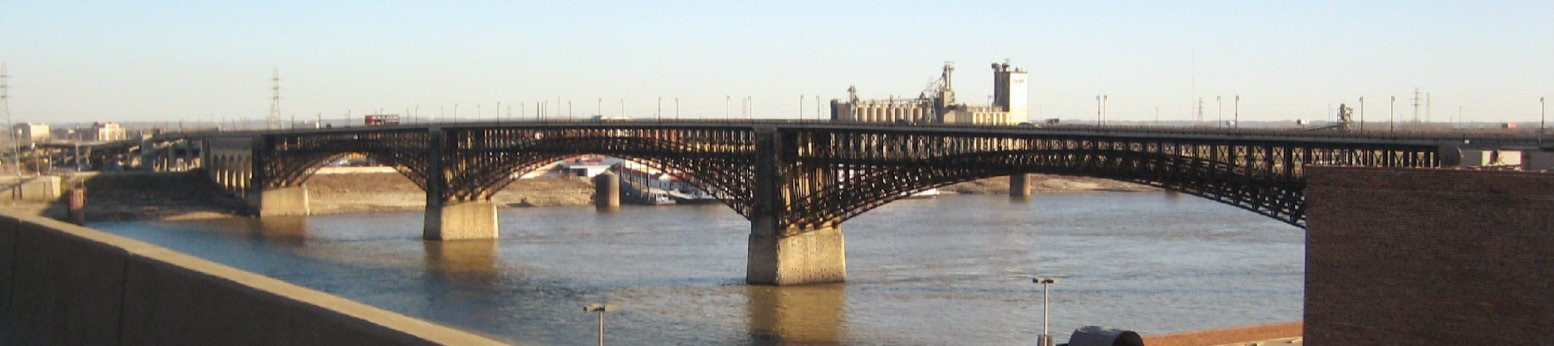
\includegraphics[width=\linewidth]{eads-bridge2.jpg}
  % \caption{Eads Bridge. (Courtesy KTA-Tator, Inc.)}
  \caption{伊兹桥}
  \label{fig:eads-bridge2}
\end{figure}

After about 1965, bridge coating engineers began to turn away from coatings containing these toxic “heavy
metal” pigments and instead started using coatings containing metallic zinc as the corrosion-inhibitive pigment. The
DOT survey conducted as part of the SHRP 2 R19A Project (final report forthcoming) indicated that all states
responding use a system consisting of a zinc-rich primer. As long as the zinc pigment in the coating is in close metalto-
metal contact with the steel substrate, the coating provides galvanic protection to the steel. Galvanic protection is
provided when zinc and steel (iron) are connected (i.e., have a conductive pathway between them) with one another in the presence of air (oxygen) and moisture. In this coupling of materials, zinc (the less noble metal) will oxidize
(corrode) in preference to the iron (steel). The preferential oxidation of zinc provides protection for the steel as long
as there is nearby zinc left to be consumed in the chemical reaction which takes place at the anode. When the zinc is
consumed, the steel beneath will be subject to corrosion (oxidation). The method used to resist corrosion attack
since about the mid-1960s has been to utilize a multi-coat, “belt and suspenders,” approach. In a multi-coat system,
the outer layer(s) resist the effects of weather and protect the zinc from being consumed in the atmosphere, while the
zinc-rich primer inhibits corrosion from occurring at the steel beneath in locations where the coating is breached.

Even in instances in which steel is painted with a coating system utilizing a zinc-rich primer, when the protected
steel surface is bathed in salt water and is subjected to many wet/dry cycles, discontinuities in the coating inevitably
provide a pathway through the coating for moisture to reach the zinc-coated steel surface beneath. As a result, the
zinc begins to react to protect the steel from corroding. Eventually, the metallic zinc in the zinc-rich primer is
consumed, and corrosion in the form of red rust (iron oxide) results. The corrosion protection offered by zinc may
take many years to be consumed before evidence of corrosion of the steel; therefore, the rate of corrosion is dictated
by the local factors surrounding the steel (wet/dry cycles, chloride contamination, humidity, etc.).

The following general discussion of coatings serves as an introduction to discourse on the use of protective
coatings in the prevention of corrosion of structural steel. \cref{fig:paint-system} identifies the various items discussed.

\begin{figure}
  % \includegraphics[width=\linewidth]{graphic-file}
  \caption{Paint system general considerations}
  \label{fig:paint-system}
\end{figure}

\subsubsection{Composition of a Paint Coating}
\cref{fig:industry-coating} illustrates the basic ingredients of an industrial protective coating. The chart divides a coating into two
major components: pigmentation and vehicle. The pigmentation typically consists of corrosion inhibitors, colorants,
and extenders, although other raw materials may also be included. The vehicle typically consists of the resin or
binder, solvents, and any additives that may be included in the formulation. It may also contain other raw materials to
provide additional or different performance characteristics. The vehicle “carries” the pigmentation to the surface and
binds it into the coating film.

The ingredients can also be categorized as non-volatile components and volatile components, indicated on the
chart by (NV) and (V). Non-volatile components remain in the coating and on the surface once applied. Conversely,
the volatile components evaporate from the coating into the air once the coating is applied to the surface. The nonvolatile
components typically include the resin or binder, the pigmentation, and any additives that may be
incorporated into the formulation. The volatile component is the solvent system used in the formulation that is a
component of the wet film, but not the dry film of the coating.

\begin{figure}
  % \includegraphics[width=\linewidth]{graphic-file}
  \caption{Industrial coating elements. (Courtesy KTA-Tator, Inc.)}
  \label{fig:industry-coating}
\end{figure}


\paragraph{Vehicle Resin}
The vehicle resin (or binder) portion of the coating vehicle is comprised of both volatile a non-volatile
component. That is, it is both part of the wet film and the dry film. Often a coating is identified generically by the type of resin used in the formulation. For example, a two-coat epoxy is a commonly specified coating system. In this
case, “epoxy” is used to describe both the coating type and the raw material resin system used to formulate the
coating. The resin system is the film-forming component of a coating. It cohesively bonds the pigmentation together
and adhesively bonds the coating to the underlying substrate or coating layer. It is essentially the “glue” of the
coating. In many cases, the resin system dictates the performance properties of a coating.

\subparagraph*{Pigmentation}
The pigment is also a non-volatile component of the coating formulation and is essentially an insoluble raw
material. It suspends in the resin and solvent rather than dissolving. While some feel that the pigment merely gives
the coating its color that is only one of several potential functions.

The pigment in a coating may also provide corrosion protection. If so used, the pigmentation must be formulated
into the primer layer (the layer adjacent to the steel substrate). Inhibitors like barium, phosphorous, and others
formulated into a primer inhibit the corrosion process. Zinc powder added to a primer in sufficient quantities
galvanically protects the underlying steel. Because of the shape, certain pigments even provide barrier protection; in
other words, their inherent shape and the way in which they orient themselves in the dry film, create a barrier to
moisture penetration through the coating. Examples include micaceous iron oxide and leafing aluminum pigments.
These raw materials are lamellar, meaning they are plate-like, tend to lie flat in the coating film, and cause any
moisture that penetrates the coating film to take a considerably longer pathway to the substrate. Extenders such as
silica, mica, and clay may be incorporated into the formulation to improve film build; increase the solids content of
the coating, and/or provide added barrier protection.

\subparagraph*{Additives}
Additives formulated into the coating also become part of the dry film. Various quantities of additives are used
by the formulator to adjust the consistency, flow-out, surface wetting, color, ultraviolet (UV) light (sunlight)
resistance and flexibility, or to prevent settling in the can (suspending agents). For example, an alkyd coating that
typically chalks and fades upon exposure to sunlight can be formulated with silicone (minimum 30\%) to provide
better color and gloss retention characteristics. In this case, the silicone is an additive. Polyurethane coatings are formulated with hindered amine light stabilizers (HALS) to help preserve gloss and color upon exposure to sunlight,
and plasticizers formulated into a coating provide film flexibility.

\subparagraph*{Solvents}
The solvent system in a coating is the volatile component. While the solvent system is part of the wet film during
application, it is not intended to be part of the dry film once the coating dries or cures. This component is referred to
as a solvent system because it is uncommon for a coating to be formulated with but one type of solvent. Typically, a
blend of solvents is used, and each type of solvent in the blend may perform a different function. As a general rule,
primary solvents are formulated into the coating to reduce the viscosity of the resin, pigment, and additives, so that
the coating can be properly atomized through a spray gun, or applied by brush and roller. Secondary solvents
typically stay in the wet coating film a little longer than the primary solvents, as they are more slowly evaporating
solvents, and help the coating to flow-out to form a uniform, continuous film.

\subparagraph*{Volatile Organic Compounds (VOCs)}
Solvents have been used in coatings for many decades, as they have been useful and affordable. Many solvent
systems in a coating (and thinners added to a coating by the applicator) are categorized as volatile organic
compounds by the Environmental Protection Agency (EPA). Therefore, the type and amount of solvent(s) used in an
industrial coating may be regulated by the EPA because as they evaporate from the coating film into the air, they can
photochemically react with sunlight and become a precursor to ozone (a component of smog). Federal and state
environmental agencies have developed regulations to control ozone-producing operations as part of the Clean Air
Act. The amount of VOCs that can be legally emitted into the atmosphere varies considerably from location to
location. For example, densely populated areas like Southern California and Houston, Texas, have very strict VOC
regulations, while less populated areas typically comply with the federal limit, which represents a considerably
higher threshold. California has led the nation in the march toward coatings with ever-lower amounts of VOCs.
Coatings suppliers have been reformulating and retesting their coatings as VOC regulations have tightened, and
eventually, the use of such materials in coatings may diminish to the point that they are not a significant part of
coatings used on bridges.

The VOC content of a coating is expressed in pounds per gallon (or grams per liter), and is reported on the
manufacturer’s product data sheet (PDS). Many manufacturers also recalculate the VOC content of a coating after the
addition of thinner and this information is also commonly referenced on the PDS.

When painting a structure in the field, the VOC limit is typically dictated by the specification or the local air
pollution agency for the project. Conversely, fixed facilities such as painting shops are sometimes required to log the
number of gallons of paint used over a specific period (say 90 days) and the VOC content of each type.

\subsubsection{Curing Mechanisms}
The method in which a coating converts from a liquid to a solid state is known as the curing mechanism. Many
liquid-applied coatings dry by solvent evaporation, but cure by employing a separate reaction.

\paragraph{Solvent Evaporation}
Coatings that cure by solvent evaporation actually only dry. That is, the resin, pigment, and additives are
suspended in a solvent system. When the solvent evaporates from the applied film into the air, the resin, pigment, and
additives remain on the surface. Because there is no subsequent curing reaction, the resin can be re-dissolved by the
solvent system that evaporated from the coating film. That is why a coating that cures by solvent evaporation should
not be over-coated with a coating containing strong solvents, as such solvents may re-dissolve the underlying coating
film. A vinyl coating is an example of a coating that cures by solvent evaporation.
\paragraph{Coalescence}
Waterborne acrylic coatings cure by solvent evaporation and form a coating film by a process known as
coalescence. Water, the primary solvent in these coatings, first evaporates from the acrylic-containing emulsion
coating film. As the water evaporates, a special coalescing solvent (e.g., propylene glycol) aids in fusing the acrylic
emulsion particles together to form a solid film. The coalescing solvent then evaporates from the coating film.
Without this coalescing solvent, the acrylic particles will not impinge and fuse together; this can result in a poor
performing coating film. Note that the coalescing process typically requires a minimum 50°F air temperature. Should
the air temperature fall below 50°F before the coalescing process is complete, curing may stop and may not start
again once the temperature recovers. This major concern with industrial waterborne acrylic coatings should be
carefully considered by the would-be specifier.

\paragraph{Oxidation}
Coatings that cure by oxidation react with oxygen (air) to form a film. This oxidation process never stops as long
as the coating is exposed to oxygen. For example, long-used alkyd coatings, which typically contain unsaturated oils,
pigments, and driers, cure by oxidation. Many aged alkyd systems, even those that have been in service for decades,
become very brittle, as the resin continues to oxidize long after the coating is fully cured.
\paragraph{Polymerization}
The prefix “poly” means “many.” Many monomers or “mers” are used to create a polymer. These monomers are
formulated into components, and the components are packaged by the coating manufacturer separately. It is only
when these components are blended together in the correct proportions that a chemical reaction known as
polymerization occurs, generating a very resilient coating layer. Coatings that cure by polymerization are multicomponent,
typically two or three containers. Prior to application, these components are blended together in the
correct ratio. Generally, only complete, pre-packaged kits are blended. Once blended, the chemical reaction begins.
Coatings that cure by polymerization have a limited pot life. That is, the blended components must be applied before
that pot life expires. The pot life will vary from a few minutes to several hours, depending on the formulation and
temperature of the coating. Many coatings cure by polymerization; epoxy coatings and aliphatic acrylic or polyester
polyurethane coatings are a few of the more common types used on bridges.

\paragraph{Moisture Cure}
Hydrolysis is the reaction of a coating with moisture in order to cure. Only a few industrial coatings hydrolyze in
the curing process. These include moisture-cure urethanes and ethyl silicate-type inorganic zinc-rich primers, which
require a minimum amount of moisture to cure. In this process, moisture-cure urethanes release carbon dioxide
(CO2), and inorganic zinc-rich primers release ethyl alcohol. The moisture cure process results in a very resilient
coating layer, similar to that achieved by polymerization. (Zinc coatings are further discussed in a subsequent
section.)

\subsubsection{Coating Systems Defined}
In many cases, coatings can be combined to create a coating system, which includes both the surface preparation
and the application of one or more coating layers. If multiple coats of the same product are specified, contrasting
colors are sometimes used to help ensure the coverage of the applicator.

Although coating layers usually consist of a primer and topcoat, in many instances an intermediate coat may also
be specified. When multiple coatings are used to create a system, they must be compatible. In addition, each coating
layer has a function that is performed at a given thickness. Accordingly, adding extra thickness of an epoxy
intermediate coat cannot make up for an inadequate zinc-rich primer thickness. Each layer should be applied at the
optimum thickness (i.e., neither too thick nor too thin) and verified for proper thickness prior to the application of
subsequent layers.

\paragraph{Surface Preparation}
The Society for Protective Coatings (SSPC) and NACE International (NACE) have developed standard
requirements that include the end condition of the surface and materials and procedures necessary to achieve and
verify the end condition.

The level of surface preparation to be performed is an integral component to the coating system. For example,
there would be little point in applying a zinc-rich primer to a marginally-prepared surface, since the zinc must
maintain intimate contact with clean steel to provide galvanic protection. If zinc were to be applied over an old
coating, the desired galvanic protection cannot develop. Conversely, applying a surface-tolerant coating to a surface
prepared to SSPC-SP 5/NACE No. 1, White Metal Blast Cleaning, is overkill, as equivalent performance could be
achieved over a much lesser degree of cleaning, usually at a much lower cost.

\paragraph{Primer Function}
The function of the primer is to bond the coating system to the substrate. It also provides corrosion protection for
the steel substrate using one or more methods of barrier, inhibitive, or galvanic protection. The primer must also be
tolerant of the level of surface preparation performed and must be compatible with the next layer applied. If the
primer is the only layer, as with a single coat system, it must be resistant to the service environment and provide
corrosion protection to the steel beneath.


\paragraph{Intermediate Coat Function}
An intermediate coat is typically incorporated into a coating system for the purpose of adding barrier protection.
It must be compatible with both the primer and the topcoat.

\paragraph{Topcoat Function}
The topcoat, or finish coat, is the first line of defense in a corrosion protection system. It must also be
aesthetically compatible with the specifier’s priorities and is often required to maintain color and gloss levels for long
periods of time. Naturally, the topcoat must be resistant to the service environment, and must be compatible with the
underlying layer (i.e., primer or intermediate coat, as appropriate). In addition, the topcoat must be able to accept a
maintenance overcoat.

\subsubsection{Coating Application Methods}

\paragraph{Conventional (Air) Spray}
Conventional or “air-atomized” spray uses compressed air to transport the paint from a pressurized pot to the
spray gun, in order to atomize the coating into a fine spray and then propel the atomized coating to the surface. As
the ratio of air to paint is quite high (~600:1), compressed air cleanliness is critical and transfer efficiency is
relatively low. The primary reason conventional (air) spray is used to apply industrial coatings is the ability to
precisely control the amount of paint that exits the spray gun and to control the shape of the spray pattern. The
apparatus used for the application of metalizing spray is a special variation of a conventional spray gun.

Conventional air spray equipment consists of a pressure pot equipped with two regulators. The first is used to
control the amount of pressure in the pot itself, known as pot pressure, and the other is used to control the volume of
atomization air that is used to break up the stream of paint exiting the spray tip. Coating manufacturers provide
recommended pot and atomization pressures, which often have to be adjusted slightly based on project conditions
(e.g., amount of thinner addition, temperature, etc.). Two hoses connect the spray gun to the pot; one containing the
paint and the other contains the atomization air. The spray gun has two controls. The lower control regulates the
amount of paint that comes out of the spray tip, and essentially adjusts how far the operator can pull back the spray
gun trigger, which regulates the amount of paint that exits the spray tip. The upper control regulates the shape of the
fan pattern from a small circle for striping of corners, etc. to a larger oval for spraying flat surfaces. A conventional
spray gun can be half-triggered—that is, the trigger can be pulled back part way—so that the atomization air, without paint, exits the spray nozzle. This compressed air can be used to perform a final blow-down of the surface
immediately prior to coating application.

The conventional spray gun is held 6-10 in. from the surface, with variations in distance dependent on the type of
coating and prevailing spraying conditions, such as air temperature and wind speed.

\paragraph{Airless Spray}
Airless spray has long been the most common method used for applying bridge coatings. If the equipment is
operating properly and the applicator employs good spray technique, the finish quality can approach that which is
created by conventional spray, but at much higher production levels. Because airless spray does not use compressed
air to atomize the coating, the transfer efficiency is relatively higher than conventional spray, reducing airborne
emissions. Further, because airless spray does not incorporate compressed air into the paint stream, the cleanliness of
the compressed air is not critical.

Airless spray equipment consists of a paint pump that is operated using an air compressor equipped with a
regulator. Coating manufacturers provide recommended airless spray pressures, which frequently have to be adjusted
slightly based on project conditions such as amount of thinner addition, temperature, etc. A single hose containing
the paint connects the spray gun to the pump.

The airless spray gun is held 18-24 in. from the surface is, with variations in distance dependent on the type of
coating and prevailing spraying conditions.

\paragraph{Plural Component Spray}
Plural component spray is used for coating materials with a relatively short pot life or coating materials that do
not have viscosity-reducing solvents in them (e.g., 100\% solids materials). Plural component spray does not require
pre-mixing the coating components. Rather, the individual components are pumped to a mixer/manifold at the correct
ratio, then are mixed and delivered to the spray gun using a short material hose that can be flushed with solvent using
a solvent purge system. This is known as an internal mix process. There are also external mix plural component
systems that send each component to the spray gun in separate material hoses. The components blend as they exit the
spray tip. It is common for the material hoses to be heated for plural component spray, in order to reduce the
viscosity of the components and allow for easier transport and improved atomization.

Plural component spray is available in two basic designs: fixed ratio and variable ratio proportioning pumps.
Fixed ratio pumps can only proportion the components in a set ratio (e.g., 1:1), while a variable ratio pump can
proportion the materials according to the required ratio (e.g., 2:1, 4:1, 8:1, 16:1). Plural component spray equipment
can be complex and typically requires a technician to set up the equipment and monitor the mix ratio, so that the
coating materials are not applied off-ratio. This equipment is set up to spray similar to airless.

\paragraph{Electrostatic Spray}
Electrostatic spray is sometimes used to apply bridge coatings. Because of its potentially high transfer efficiency
rate, and the resulting reduction in material usage, it can be an attractive application method. In principal, the paint
particles are energized (+) as they exit the spray gun. The electrical charge is imparted by a small wire protruding
from the spray nozzle. The surface to be coated is grounded (-). The particles are “attracted” to the component or part
having the opposing electrical charge, significantly reducing overspray and material usage. The coating, however,
must be able to accept an electrical charge, and the addition of a polar solvent is sometimes required to inhibit the
coating’s natural resistivity. Electrostatic spray can also result in a wrapping of the coating on the opposite side of the
direction of spray, making it an attractive alternative for coating inaccessible areas. Because of the difficulty in
achieving a uniform ground on large structures, electrostatic spray has not been widely used to coat bridges.
Electrostatic spray equipment is typically set up to spray as an airless operation, and electrostatic spray can be used to
coat smaller members and hard-to-reach areas.

\paragraph{Brushes, Rollers, and Daubers}
The use of brushes for bridge projects is typically limited to striping—the application of a layer of coating to
surfaces where it is difficult to achieve a normal film build. For the same reason, brushes are also used on pitted or
rough surfaces around rivet heads, welds, and bolt and nut assemblies, and to cut-in inside and outside corners.
Daubers are often used to coat surfaces within crevices like back-to-back angles. Rollers have high coating transfer
efficiency and can be used to coat large flat surfaces with limitations: roller nap can become embedded in the dry
coating film and act like a wick to pull moisture into the coatings and film thickness is hard to control with a roller.

Choosing the method of coating application depends on many factors including the size and configuration of the
surfaces to be coated, the proximity to other structures, environmental regulations, and the specification and the coating manufacturer’s recommendations. While airless spray is no doubt the most frequently utilized method, there
are other issues for the contractor/applicator to consider when choosing an application method, including speed and
control.

\subsection{Description of Coating: Hot-Dip Galvanizing (HDG)}
Hot-dip galvanizing is the process in which fabricated steel, structural steel, castings, or small parts, including
fasteners, are immersed in a kettle or vat of molten zinc, resulting in a metallurgically-bonded alloy coating that
protects the steel from corrosion. HDG is often referred to as simply “galvanizing.” The term is often used
incorrectly to describe steel coated with zinc by other methods such as paint or plating. All of these methods of
applying zinc to steel for corrosion protection are very different from HDG.

HDG forms a metallurgical bond between the zinc and the underlying steel or iron, creating a barrier that is part
of the metal itself. During galvanizing, the molten zinc reacts with the surface of the steel or iron article to form a
series of zinc/iron alloy layers. \cref{fig:cross-section-galvanized-coating} is a photomicrograph of a galvanized steel coating cross-section and
shows a typical coating microstructure.

The HDG coating consists of four separate layers. The first three layers have a mixture of iron and zinc, and the
external top layer is typically composed of 100\% zinc.

\begin{figure}
  % \includegraphics[width=\linewidth]{graphic-file}
  \caption{Magnified cross-section of galvanized coating}\label{fig:cross-section-galvanized-coating}
\end{figure}

Below the name of each layer in \cref{fig:cross-section-galvanized-coating} is its respective hardness, expressed by a Diamond Pyramid Number
(DPN). The DPN is a progressive measure of hardness; the higher the number, the greater the hardness. Typically, the Gamma, Delta, and Zeta layers are harder than the underlying steel. The hardness of these inner layers provides
unusual protection against coating damage by abrasion. The Eta layer is quite ductile, providing the coating with
some impact resistance. The galvanized coating is adherent to the underlying steel on the order of several thousand
pounds per square in. (psi). Hardness, ductility, and adherence combine to provide the galvanized coating with
unmatched protection against damage caused by rough handling during transportation to the project site, and/or at the
project site, as well as while in service. The toughness of the galvanized coating is extremely important since barrier
protection is dependent upon the integrity of the coating.

\subsubsection{The HDG Process}

Though the process may vary slightly from plant to plant, the fundamental steps in the galvanizing process are
surface preparation, galvanizing, and finishing.

\paragraph*{Surface Preparation}

\begin{description}
  \item[Degreasing/Caustic Cleaning] A hot alkaline solution removes dirt, oil, grease, shop oil, and soluble markings.
  \item[Pickling] Dilute solutions of either hydrochloric or sulfuric acid remove surface rust and mill scale to provide a
  chemically clean metallic surface.
  \item[Fluxing] Steel is immersed in liquid flux, usually a zinc ammonium chloride solution, to remove oxides and
  prevent oxidation prior to dipping into the bath of molten zinc. In the dry galvanizing process, the item is separately
  dipped in a liquid flux bath, removed, allowed to dry, and then galvanized. In the wet galvanizing process, the flux
  floats on top of the molten zinc and the item passes through the flux immediately prior to galvanizing.
\end{description}

\paragraph*{Galvanizing}
The article is immersed in a bath of molten zinc between 815°F to 850°F (435°C to 455°C). During galvanizing,
the zinc metallurgically bonds to the steel, creating a series of highly abrasion-resistant zinc–iron alloy layers,
commonly topped by a layer of impact-resistant pure zinc.

\paragraph*{Finishing}
After the steel is withdrawn from the galvanizing bath, excess zinc is removed by draining, vibrating, or, in the
case of small items, centrifuging. The galvanized item is then air-cooled or quenched in liquid.

\subsubsection{Coating Uniformity}
The galvanizing process produces coatings that are at least as thick at the corners and edges as the coating on the
rest of the article. As coating damage is most likely to occur at the edges, this is where added protection is needed
most. \cref{fig:galvanized-corner} is a photomicrograph showing a cross-section of a corner of a galvanized piece of steel.

\begin{figure}
  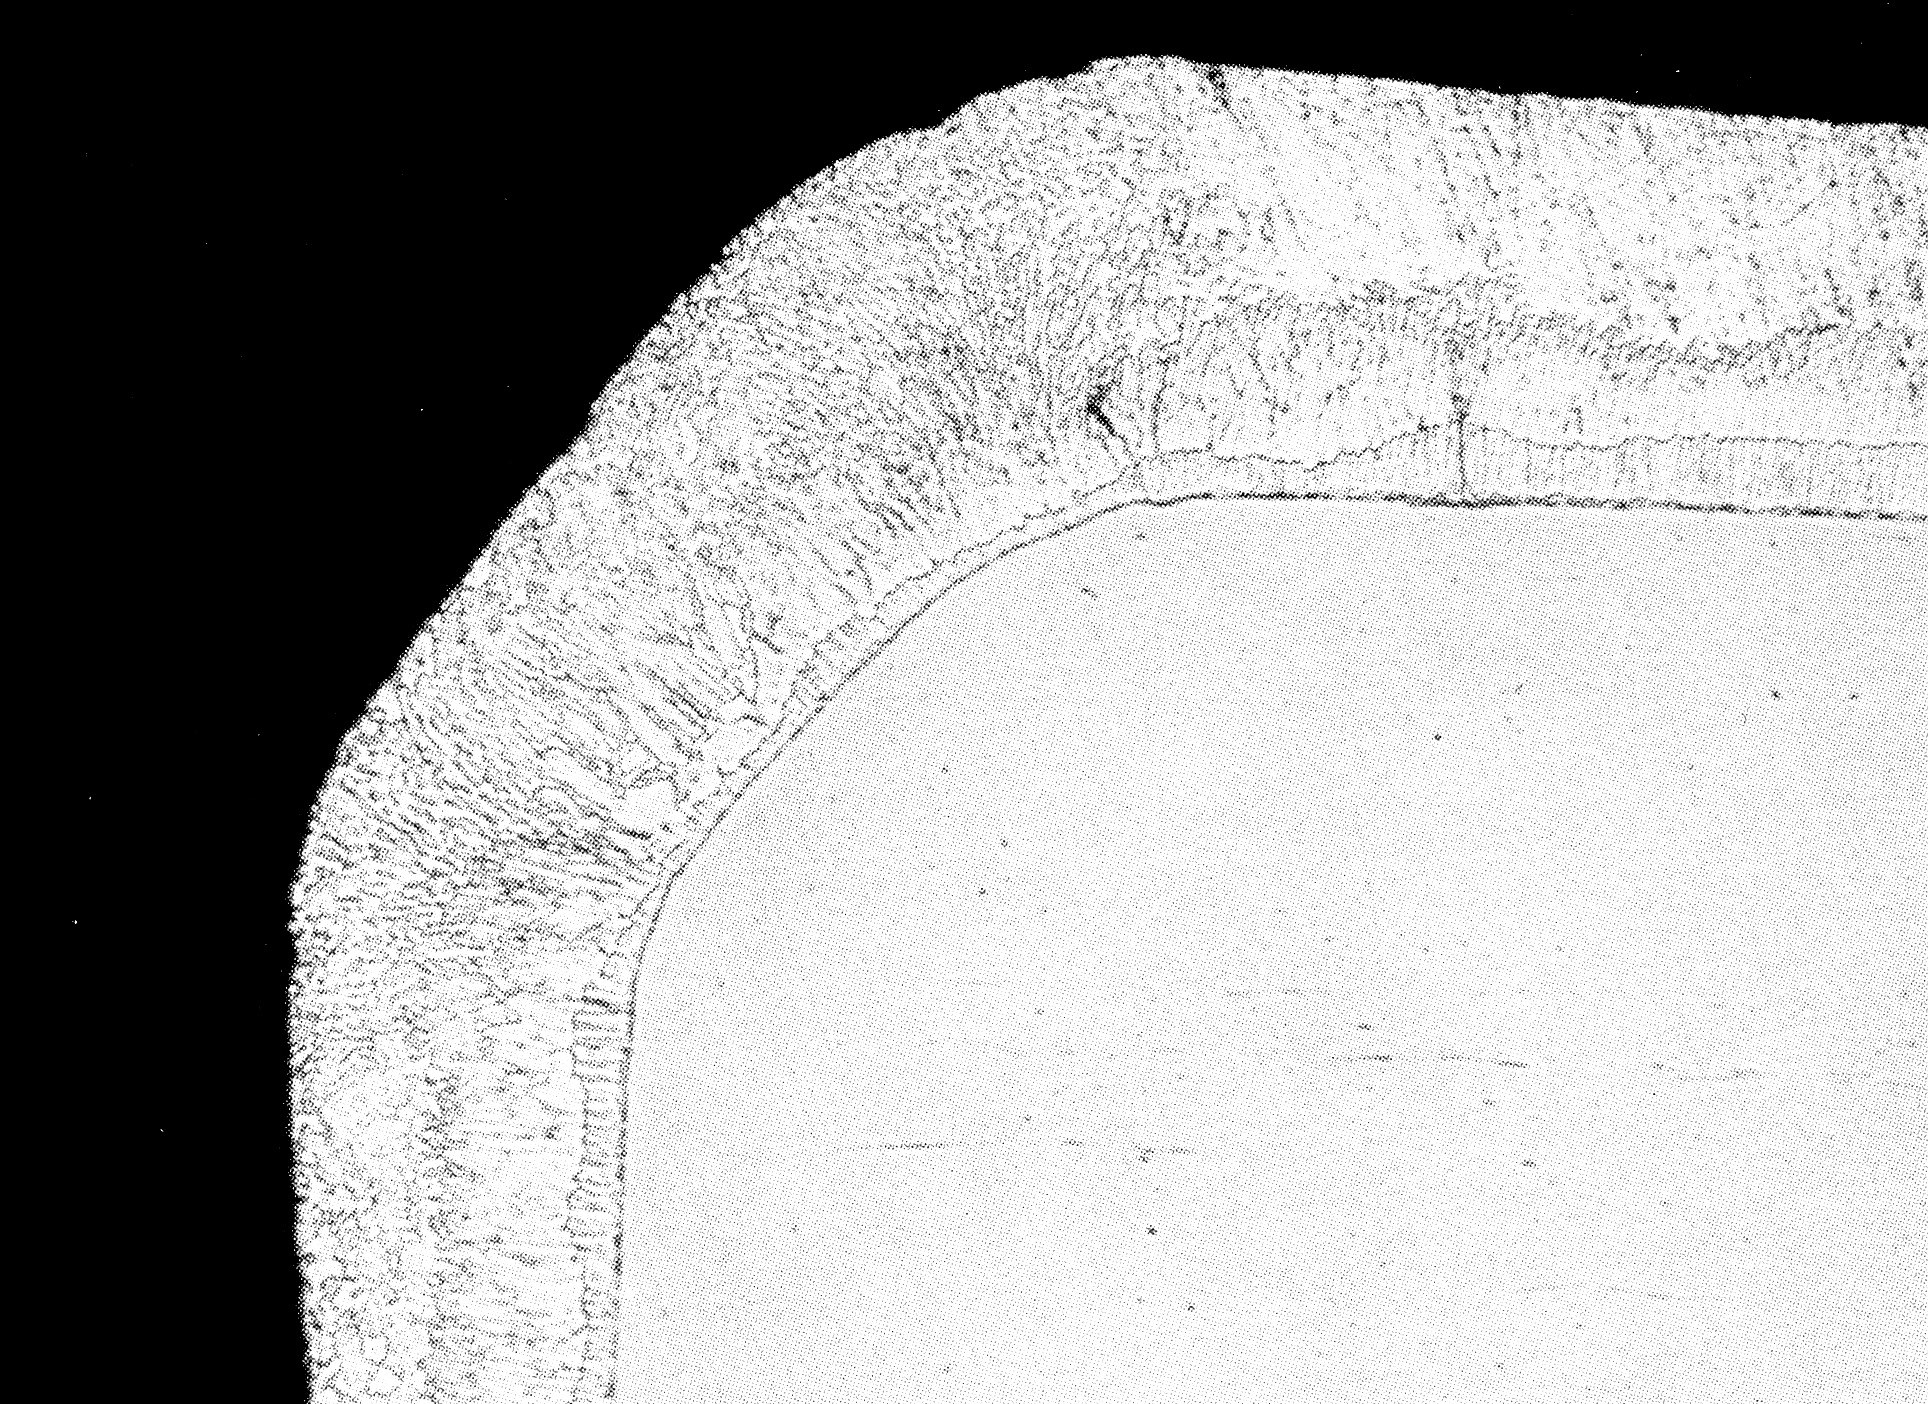
\includegraphics[width=0.4\linewidth]{galvanized-corner.jpg}
  % \caption{Cross-section of corner of galvanized steel section. (Courtesy American Galvanizers Association)}
  \caption{镀锌钢型材转角的横截面}
  \label{fig:galvanized-corner}
\end{figure}

Because the galvanizing process involves total immersion of the material, all surfaces are coated. Galvanizing
provides protection on both exterior and interior surfaces of hollow structures, which must be detailed in a way that
allows zinc to drain from the interior when the item is removed from the kettle.

The inspection process for galvanized items is straightforward and requires minimal labor. Galvanizing takes
place in a factory regardless of weather or humidity conditions. The galvanizer’s ability to work in any type of
weather provides a higher degree of assurance of on-time delivery and a turnaround time of two or three days is
common.

The American Society of Testing and Materials International (ASTM), the Canadian Specification Association
(CSA), and the American Association of State Highway and Transportation Officials (AASHTO) specifications
establish minimum standards for thickness of galvanized coatings on various categories of items. These minimum
standards are routinely exceeded by galvanizers due to the nature of the galvanizing process, which includes factors
that influence the thickness and appearance of the galvanized coating such as chemical composition of the steel, steel surface condition, cold-working of steel prior to galvanizing, bath temperature, bath immersion time, bath withdrawal
rate, and steel cooling rate.

\subsubsection{Effect of Amount of Silicon in Steel on Galvanize Coating}
The chemical composition of the steel being galvanized is very important and the amount of silicon and
phosphorus in the steel strongly influences the thickness and appearance of the galvanized coating. Silicon,
phosphorus, or combinations of the two elements can cause thick, brittle galvanized coatings. The coating thickness
curve shown in \cref{fig:galvanize-coating-thickness-curve} relates the effect of silicon in the base steel to the thickness of the zinc coating. The
carbon, sulfur, and manganese content of the steel also may have a minor effect on the galvanized coating thickness.

\begin{figure}
  % \includegraphics[width=\linewidth]{graphic-file}
  \caption{Galvanize coating thickness curve. (Courtesy American Galvanizers Association)}\label{fig:galvanize-coating-thickness-curve}
\end{figure}

The combination of elements mentioned, known as “reactive steel” in the galvanizing industry, tends to
accelerate the growth of zinc-iron alloy layers. This may result in a finished galvanized coating consisting entirely of
zinc-iron alloy. Instead of a shiny appearance, the galvanized coating has a dark gray, matte finish that will provide
as much corrosion protection as a galvanized coating having a bright appearance.

It is difficult to provide precise guidance in the area of steel selection for galvanizing; however, the guidelines
discussed below usually result in the selection of steels that provide good galvanized coatings.

\begin{itemize}
  \item Carbon levels less than 0.25\%, phosphorus less than 0/04\%, or manganese less than 1.35\% are beneficial,
  \item Silicon levels less than 0.03\% or between 0.15\% and 0.25\% are desirable.
\end{itemize}

Although it is not part of the controlled composition of the steel, silicon may be present in many steels
commonly galvanized. This occurs primarily because silicon is used in the de-oxidization process in making steel
and is found in continuously-cast steel. The phosphorus content should never be greater than 0.04\% for steel that is
intended for galvanizing. Phosphorus acts as a catalyst during galvanizing, resulting in rapid growth of the zinc-iron
alloy layers. This growth is virtually uncontrollable during the galvanizing process.

As the galvanizing reaction is a diffusion process, higher zinc bath temperatures and longer immersion times will
generally produce somewhat heavier alloy layers. Like all diffusion processes, the reaction proceeds rapidly at first
and then slows as layers grow and become thicker. However, continued immersion beyond a certain time will have
little effect on further coating growth. When galvanizing reactive steels, the diffusion process proceeds at a faster
rate, producing thicker coatings.

The thickness of the outer pure zinc layer is largely dependent on the rate of withdrawal from the zinc bath. A
rapid rate of withdrawal causes an article to carry out additional zinc and generally results in a thicker coating.

ASTM, CSA, and AASHTO specifications and inspection standards for galvanizing recognize that variations occur in both coating thickness and compositions. Thickness specifications are stated in average terms. Further coating thickness measurements must be taken at several points on each inspected article to comply with ASTM A123/A 123M for structural steel and A 153/A 153M for hardware. \cref{fig:coating-thickness-measuring} shows thickness measurement being taken.

\begin{figure}
  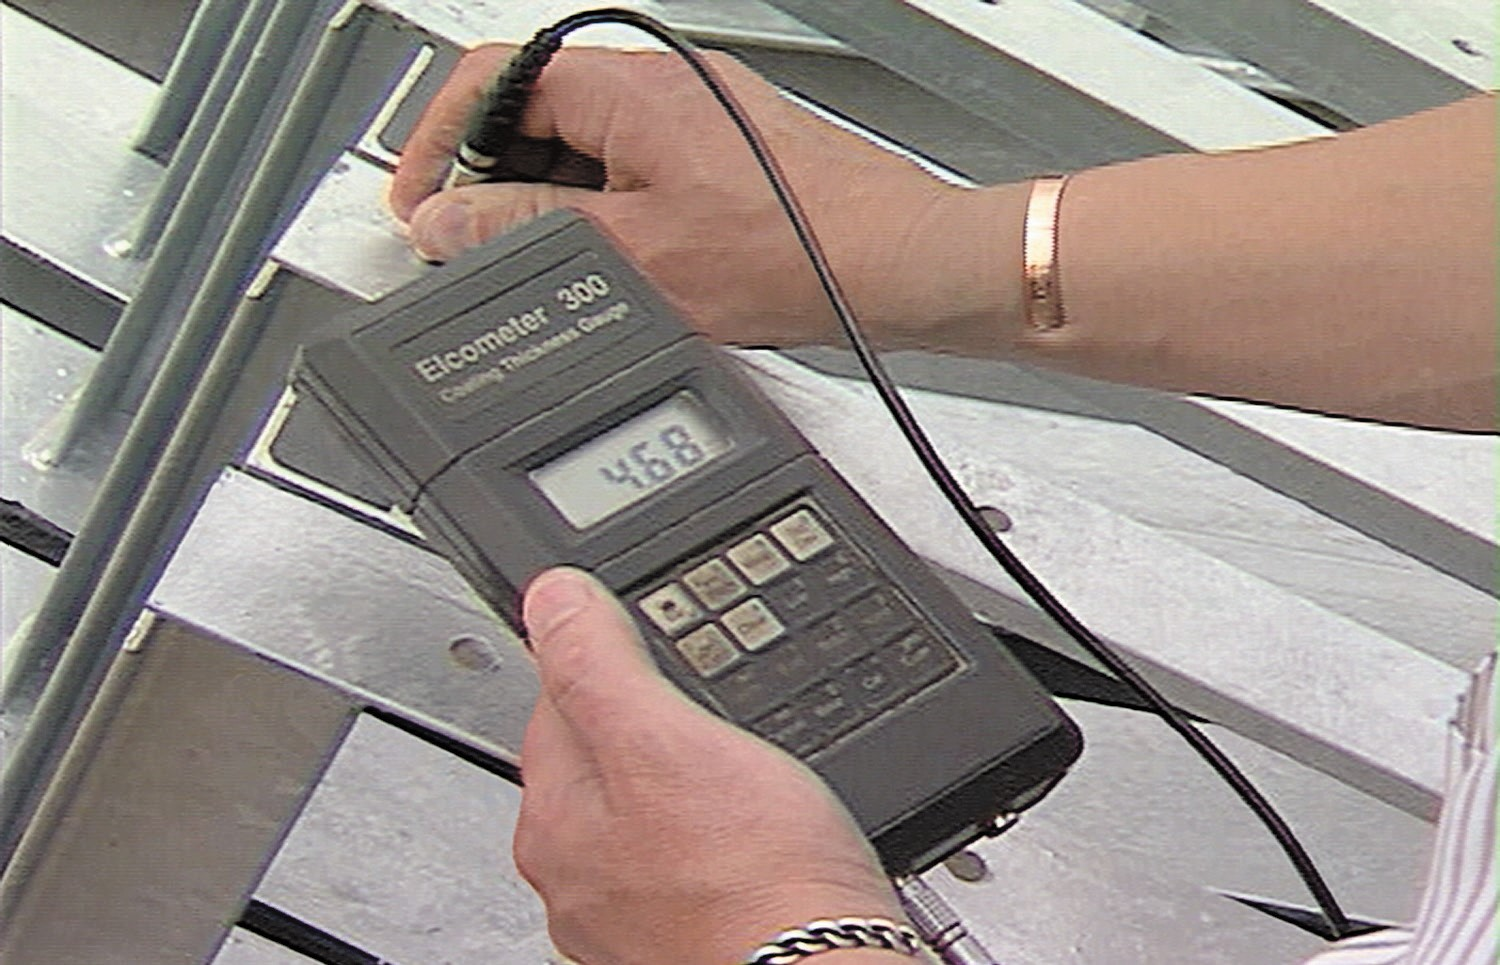
\includegraphics[width=0.65\linewidth]{coating-thickness-measuring.jpg}
  % \caption{Coating thickness measuring. (Courtesy American Galvanizers Association)}
  \caption{涂层厚度测量}
  \label{fig:coating-thickness-measuring}
\end{figure}

Fortunately, many grades of steel commonly used in steel bridges meet the chemical requirements and are readily
galvanized. When in doubt the owners/engineers should be queried and/or the galvanizer’s advice should be sought.

% \subsubsection{Inspection}
\subsubsection{检查}

Inspections for coating thickness and surface condition complete the process. Inspection of structural steel will
normally fall under ASTM A123/A123M—12 Standard Specification for Zinc (Hot-Dip Galvanized) Coatings on
Iron and Steel Products or ASTM A153/A153M—09 Standard Specification for Zinc Coating (Hot-Dip) on Iron and
Steel Hardware.

\subsection{Description of Coating: Thermally Sprayed Metal Coating (TSMC) or Metalizing}
When sizes and shapes of steel members will not fit in a galvanizing kettle or when the schedule simply does not
allow time to transport items to a galvanizer’s plant, there is the option to metalize the item.

Thermally sprayed metal coating, referred to as metalizing, is the process of applying metallic zinc in wire form
to clean steel by feeding it into a heated gun, where it is heated, melted, and spray applied by using combustion gages
or auxiliary compressed air to provide ample velocity. Metalizing may be used on any size steel object, thereby
eliminating limitations due to vat size and awkward shapes. Applying a consistent coating in recesses, hollows, and
cavities adds a measure of complexity. Pure zinc can be used, but often zinc is alloyed with 15\% aluminum to
provide a smoother abrasion resistant film.


\subsubsection{TSMC Processes}
Two similar processes are used to apply the metallic zinc to the steel surface. These are differentiated by the
manner in which the zinc metal is melted as described in the following sections.
\paragraph*{Flame Spray Process.}
The flame spray process can be used to apply a wide variety of feedstock materials, in addition to metal wires
including ceramic rods, and metallic and nonmetallic powders. In flame spraying, the feedstock material is fed
continuously into the tip of the spray gun or torch, where it is then heated and melted in a fuel gas/oxygen flame and
accelerated toward the substrate being coated in a stream of atomizing gas. Common fuel gases used include  acetylene, propane, and methyl acetylene-propadiene (MAPP). Oxyacetylene flames are used extensively for wireflame
spraying because of the degree of control and the higher temperatures attainable with these gases. The lowertemperature
oxygen/propane flame can be used for melting metals such as aluminum and zinc. The basic
components of a flame spray system include the flame spray gun or torch, the feedstock material and a feeding
mechanism, oxygen and fuel gases with flow meters and pressure regulators, and an air compressor and regulator.

In wire-flame spraying, the wire-flame spray gun or torch, shown in \cref{fig:flame-wire-spray-gun}, consists of a drive unit with
motor and drive rollers for feeding the wire, and a gas head with valves, gas nozzle, and an air cap that controls the
flame and atomization air. Compared with wire-arc spraying, wire-flame spraying is generally simpler and less
expensive. Both flame spraying and wire-arc spraying systems are field portable and may be used to apply quality
metal coatings for corrosion protection.

\begin{figure}
  % \includegraphics[width=\linewidth]{graphic-file}
  % \caption{Schematic of a typical flame-wire spray gun. (Figure reprinted with permission from NCHRP Report 528: Thermally Sprayed Metal Coatings to Protect Steel Pilings: Final Report and Guide. [Ellor et al., 2004])}
  \caption{典型的火焰丝喷枪示意图}
  \label{fig:flame-wire-spray-gun}
\end{figure}


\paragraph*{Wire-Arc Process}
Due to its high deposition rates, excellent adhesion, and cost-effectiveness, wire-arc spray is the preferred
process for applying TSMCs to steel bridges. In the wire-arc spray process, two consumable wire electrodes of the
metal being sprayed are fed into a gun such that they meet at a point located within an atomizing air, or other gas,
stream. An applied DC potential difference between the wires establishes an electric arc between the wires that melts their tips. The atomizing air flow subsequently shears and atomizes the molten droplets to generate a spray pattern of
molten metal directed toward the substrate being coated. Wire-arc spray is the only thermal spray process that
directly heats the material being sprayed, a factor that contributes to its high energy efficiency.

The wire-arc spray system consists of a wire-arc spray gun or torch (shown in \cref{fig:wire-arc-spray-gun}), atomizing gas, flow
meter or pressure gauge, a compressed air supply, DC power supply, wire guides/hoses, and a wire feed control unit.
Operation of this equipment must be in strict compliance with the manufacturer’s instructions and guidelines.

\begin{figure}
  % \includegraphics[width=\linewidth]{graphic-file}
  % \caption{Schematic of a typical wire-arc spray gun. (Figure reprinted with permission from NCHRP Report 528: Thermally Sprayed Metal Coatings to Protect Steel Pilings: Final Report and Guide. [Ellor et al., 2004])}
  \caption{典型的线弧喷枪示意图}
  \label{fig:wire-arc-spray-gun}
\end{figure}

\subsubsection{TSMC Guidelines}
\cref{tab:tsmc-coating-guide} provides a thermal sprayed metal coating selection guide for 20- to 40-year life, and shows the TSMC
thickness typically applied under various environmental conditions.

\begin{table}
  % \caption{TSMC Coating Guide. (National Cooperative Highway Research Program, Report 528 [Ellor et al. 2004])}
  \caption{TSMC Coating Guide}
  \label{tab:tsmc-coating-guide}
  % \input{tables/tsmc-coating-guide}
\end{table}

TSMCs should always be applied to “white” metal (SSPC-SP 5/NACE No. 1, White Metal Blast Cleaning). It is
common practice in fieldwork to apply the TSMC during the same work shift in which the final blast cleaning is
performed. The logical end point of the holding period is when the surface cleanliness degrades or a change on
performance, a bend or tensile test, for example, occurs. If the holding period is exceeded, the surface must be reblast
cleaned in order to establish the correct surface cleanliness and profile.

Thermal spraying should be started as soon as possible after the final anchor-tooth or brush blasting, and
completed within six hours for steel substrates that are subject to variations in dew point temperature or holding
period. In high-humidity and damp environments, shorter holding periods should be used.

In environments with low humidity, or in controlled environments in which enclosed structures use industrial
dehumidification equipment, it may be possible to retard the oxidation of the steel and hold the near-white-metal
finish for more than six hours. With the concurrence of the purchaser, a holding period of greater than six hours can
be validated by determining the acceptable temperature-humidity envelope for the work enclosure by spraying and
analyzing bend test coupons, tensile adhesion coupons, or both. Should the sample fail the bend test, the work must
be re-blasted and re-tested.

When specified, a flash coat of TSMC equal to or greater than 1 mil (25 um) may be applied within six hours of
completing the surface preparation in order to extend the holding period for up to four hours beyond the application
of the flash coat. The final TSMC thickness, however, should be sprayed within four hours of applying the flash
coat. This procedure should be validated using a tensile adhesion test, bend test, or both, by spraying a flash coat and
waiting through the delay period before applying the final coating thickness.

When dealing with small and movable parts, if more than 15 minutes is expected to lapse between surface
preparation and the start of thermal spraying, or if the part is moved to another location, the prepared surface should
be protected from moisture, contamination, and finger/hand marks. Wrapping the part with clean, print-free paper is
generally adequate.

If rust bloom, blistering, or a degraded coating appears at any time during the application of the TSMC, the
following procedure should be performed:

\begin{enumerate}
  \item Stop spraying;
  \item Mark off the satisfactorily sprayed area;
  \item Repair the unsatisfactory coating (i.e., remove the degraded coating and re-establish the minimum
  “white metal” finish and anchor-tooth profile depth as per the maintenance and repair procedure);
  \item Record the actions taken to resume the project in the project documentation; and
  \item Contact the coating inspector to observe and report the remedial action to the purchaser.
\end{enumerate}

The materials and application costs of a TSMC system is higher than the cost of conventional liquid-applied
coatings; however, the dominant factor may not be either material or application-labor cost. Instead, the cost of
taking the facility out of service, contractor mobilization, environmental constraints, and monitoring costs are often
the major considerations of the total cost. In some complex coating work, the actual cost of materials and application
is less than 20\% of the total process. Therefore, if service life is increased by the use of TSMC, the process can pay
for itself. Nevertheless, TSMC is used most effectively on broad flat surfaces, and complexities occur when the
gun/hoses are maneuvered around elements that are mounted at an angle to the main flat surface. For example,
TSMC is most efficient when used on a girder web or flange, but progress may be slower when connection plates or
stiffeners are encountered. The current premium for TSMC can be as little as 40\% as compared to other protective treatments. In many cases, this is a small price to pay for a material which has proven performance and an estimated
service life measured in decades.

Impact and abrasion are significant environmental stresses for any coating system. Abrasion is primarily a wearinduced
failure caused by contact of a solid material with the coating, for example foot and vehicular traffic on floor
coatings, ropes attached to mooring bitts, sand particles suspended in water, and floating ice. When objects of
significant mass and velocity move in a direction normal to the surface as opposed to parallel, as in the case of
abrasion, the stress is considered to be an impact. Abrasion damage occurs over a period of time, whereas impact
damage is typically immediate and discrete. Many coating properties are important to the resistance of impact and
abrasion including adhesion to the substrate, cohesion within the coating layers, toughness, ductility, and hardness.
Thermally sprayed coatings of zinc, aluminum, and their alloys are very impact resistant. Zinc metalizing has only
fair abrasion resistance in immersion applications because the coating forms a weakly adherent layer of zinc oxide.
This layer is readily abraded, which exposes more zinc, which in turn oxidizes and is abraded; 85:15 wt%
zinc/aluminum is more impact/abrasion resistant than pure zinc or pure aluminum.

\subsubsection{Concerns Related to Performance of the TSMC}
Coating selection may be limited by the degree or type of surface preparation that can be achieved on a particular
structure or structural component. Because of physical configuration or proximity to other sensitive equipment or
machinery, it may not always be possible to abrasive blast a steel substrate. In such cases, other types of surface
preparation, such as hand tool or power tool cleaning, may be necessary, which, in turn, may place limits on the type
of coatings that may be used. In some cases, it may be necessary to remove the old coating by means other than
abrasive blasting, such as using power tools, high-pressure water jetting, or chemical strippers. These surface
preparation methods do not impart the surface profile that is needed for some types of coatings to perform well. In
the case of thermally sprayed coatings, a high degree of surface preparation is essential. This kind of preparation can
only be achieved by abrasive blast cleaning using a good-quality, properly-sized angular blast media. Thermal
spraying should never be selected for applications in which it is not possible to provide the highest quality surface
preparation.

An angular blast media must always be used. Rounded media such as steel shot, or mixtures of round and
angular media, will not produce the appropriate degree of angularity and roughness in the blast profile. The adhesion of TSMCs can vary by an order of magnitude as a function of surface roughness profile shape and depth. TSMCs
adhere poorly to substrates prepared with rounded media and may fail in service by spontaneous delamination. Hard,
dense, angular blast media such as aluminum oxide, silicon carbide, iron oxide, and angular steel grit are needed to
achieve the depth and shape of blast profile necessary for good TSMC adhesion. Steel grit should be manufactured
from crushed steel shot conforming to SAEJ827. Steel grit media composed of irregularly shaped particles or
mixtures of irregular and angular particles should never be used. Steel grit having a classification of “very angular,”
“angular,” or “subangular,” as classified by the American Geological Institute, should be used (Hansink 1994). Also
see: Joint Standard SSPC-CS 23.00/AWS C2.23M/NACE No. 12 Specification for the Application of Thermal Spray
Coatings (Metallizing) of Aluminum, Zinc, and Their Alloys and Composites for the Corrosion Protection of Steel
(2003).

\subsection{Description of Corrosion Resistant Steels—ASTM A1010}
ASTM A1010 steel is a 10.5\% to 12.5\% chromium structural steel with superior corrosion resistance. A1010 is
widely used in thicknesses from 1/8 in. to 1/2 in. for structures subjected to aggressive service conditions, such as
coal railcars and coal processing equipment. Because of the A1010 superior corrosion resistance, it is also a
candidate for challenging bridge applications. The steel can meet the strength and impact properties of AASHTO
M270 Grades 50W and HPS 50W up to the thickness of 4 in., making it attractive steel for traditional plate girder
bridges.

\subsection{Description of Weathering Steels (WS)}

Uncoated weathering grade steels have a chemical composition containing small amounts of copper, phosphorus,
chromium, nickel, and silicon to attain their weathering or corrosion resistant properties.

Weathering grade steels are currently supplied under AASHTO Specification M270, ASTM A709 Grade 50W,
and in high performance steel grades HPS 50W, 70W, and 100W. When used in the right environment, these steels
are very cost-effective in both the short and long term as they eliminate the need for shop and field painting.

Weather steels have been successfully utilized on coal hopper cars, buildings, and electric transmission towers
and began appearing in bridges on a large scale in the mid-1960s. Currently, thousands of weather steel bridges are
providing trouble-free service across the United States.

Unpainted weather steel, properly designed and detailed, can realize bridge life cycles up to 120 years with
minimal maintenance. This high-strength, low-alloy steel forms a tightly adhering “patina” during its initial
exposure to the elements. The patina is essentially an oxide film of corrosion by-products about the same thickness
as a heavy coat of paint.

The initial corrosion of weather steel depends on the presence of moisture and oxygen. As corrosion continues, a
protective barrier layer forms that greatly reduces further access to oxygen, moisture, and contaminants. This stable
barrier layer greatly resists further corrosion, reducing it to a low value. Under appropriate conditions, weather steel
will generally corrode at a rate of less than 0.3 mils per year. Corrosion of conventional steels, on the other hand,
forms rust layers that eventually disengage from the surface, exposing fresh metal below, thereby continuing the
corrosion cycle.

Weathering steel bridges initially look orange-brown in color; however, the color will darken as the patina forms.
In two to five years, depending on the climate, the steel will attain a dark, rich, purple-brown color that many think is
attractive.

The protective patina will start to form during construction. Workers should avoid damaging the steel while it is
being stored or handled, otherwise, the weather steel will appear mottled until the patina reforms to match the
undamaged areas. If the beam ends are unpainted, constructors should wrap piers and abutments to protect them
from staining.

Bridges constructed of weathering steel in suitable environments and with proper detailing have all the qualities
of those using conventional steel and offer the following benefits:

\begin{itemize}
  \item Initial cost savings compared to conventional painted alternatives;
  \item Low maintenance consisting of periodic inspection and cleaning, which reduces direct operating costs;
  \item Minimal indirect costs from traffic delays for major maintenance operations;
  \item Faster construction resulting from elimination of shop and field painting;
  \item Good aesthetics since weathering steel bridges eventually achieve an attractive dark brown color that blends well with the environment and improves with age;
  \item Low impact on the environment compared to painted alternatives that emit undesirable volatile organic compounds;
  \item Minimal health and safety issues relating to initial and future painting; and
  \item A good track record for long-term performance based on various state and federal studies.
\end{itemize}

Several factors can impact the satisfactory performance of weather steel. Experience has shown, for example,
that weather steel requires alternating cycles of wet and dry conditions to form a properly adhering protective patina.
This would generally rule out its use in areas of high rainfall and humidity or persistent fog. Extreme marine
conditions, the presence of roadway deicing salts, pollution, surrounding vegetation, and tunnel-like conditions can
also lead to unsatisfactory performance, as can poor detailing and maintenance.

Bridge engineers should avoid specifying weather steel that will be exposed to sea water spray, salt fogs, and
immediate coastal salt environments, as salt film deposited on the metal surface, being hygroscopic, tends to maintain
continuously damp conditions, preventing the formation of a proper patina.

Heavy use of deicing salts over and under weather steel bridges may cause problems. For example, salt-laden
runoff that flows through leaking expansion joints and directly over the steel has been identified as a cause of poor
weathering steel performance.

In all probability, bridge expansion joints eventually leak, so many states recommend painting the steel beam
ends to a length 1.5 times the girder depth. Painting the ends also eliminates staining of the concrete piers below the
joints. The inclusion on the uphill end of the girder of a drip bar detail should be considered to prevent leakage from
travelling down the girder flange. Fabricators and erectors should avoid marking blast-cleaned steel with paint,
crayons, or wax, which interferes with the forming of the desired patina. Painted ends, plus the requirement to shop
blast mill scale from the weather steel to promote a uniform patina, tend to reduce the initial cost savings as
compared to painted steel. Tunnel-like conditions result from a combination of a narrow road with minimum
shoulders between vertical retaining walls or a wide bridge with minimum headroom and full-height abutments.
Such situations may be encountered at urban or suburban grade separations, in which case the lack of air currents to
dispel roadway spray leads to excessive salt deposits on the bridge girders.

In addition, weather steel bridges should not be located where ambient atmospheres contain high concentrations
of pollution and industrial fumes, especially those caused by sulfur dioxide. However, moderate industrial
environments typically speed the weathering process and more quickly achieve the mature dark color.

Detailing of weather steel bridges must promote the wet/dry cycles necessary to form the protective patina and to
avoid salt deposits on the girders. In general, the detailing should allow all parts of the steelwork to dry, avoid
moisture and debris retention, and promote adequate ventilation. For example, designers should avoid closely-spaced
girders that inhibit ventilation, and should avoid or seal overlaps and crevices that may attract moisture via capillary
action. Drainage below an overpass should prevent ponding of water, which results in continuous traffic spray.

What follows are recommendations on detailing based on those outlined in the FHWA Technical Advisory T-
5140.22, Uncoated Weathering Steel in Structures (FHWA 1989).

\begin{itemize}
  \item Eliminate bridge joints where possible through use of continuous girders and integral abutments.
  \item Control water on the deck near the expansion joints deck. Consider the use of a trough under the deck joint
  to divert water away from vulnerable elements.
  \item Paint all superstructure steel within a distance of 1.5 times the depth of girder from bridge joints.
  \item Locate welded drip bars in areas of low stress.
  \item Minimize the number of bridge deck scuppers (holes cut near the edge of a deck to drain water below). The
  use of fewer scuppers results in a higher amount of flow-through per scupper, minimizing the chances for
  blockage.
  \item Eliminate geometries that serve as water and debris traps.
  \item Hermetically seal box members when possible, or provide weep holes to allow proper drainage and air
  circulation.
  \item Cover or screen all openings in boxes that are not sealed.
  \item Consider protecting pier caps and abutment walls with drip pans and plates to minimize staining.
\end{itemize}

Designers should specify weathering grade bolts, nuts, and washers for joining weathering steel components.
Bolted connections inevitably result in crevices that can trap moisture. If detailing is such that close fit ups are
difficult, the joint could be sealed.

While the patina surface generally represents a good sign of performance, laminations and flaking are bad signs.
However, a fine-grained adherent layer indicates good expected weathering performance. Inspectors should
specifically look for leaking expansion joints, blocked drains, buildups of debris and other moisture traps, sealant
failure, and bulging joints and overlaps. If inspectors uncover any of these conditions, appropriate maintenance
should follow. In addition, research performed by Texas DOT has resulted in the following recommended measures:

\begin{itemize}
  \item Flush debris, dirt, and bird and bat droppings from the bridge structure;
  \item Clear vegetation from pier and abutment areas to enhance air circulation;
  \item Reseal deteriorating joints; and
  \item Unblock drains and troughs.
\end{itemize}

\section{Factors Adversely Affectiong Service Life}
\subsection{General}
One of the most important tasks for developing corrosion prevention systems is properly identifying the
prevailing service environment, for existing structures, or the projected service environment, for new structures.
Among the questions to be answered are, to what will the system and the bridge be subjected? In the case of a new
structure or existing structure, this can be a challenge. Service environments can be both predictable (e.g., deicing
salt exposure on a bridge in the winter) and unpredictable (e.g., hurricanes and other like storms may bring
unexpected conditions). \cref{fig:faulttree-factors-coating} shows some of the factors that can influence the service life of steel bridge
elements related to corrosion.

\begin{figure}
  % \includegraphics[width=\linewidth]{faulttree-factors-coating}
  \caption{Factors that can influence service life of coatings.}
  \label{fig:faulttree-factors-coating}
\end{figure}

The following is a brief description of environmental effects shown in \cref{fig:faulttree-factors-coating}.

\begin{description}
  \item[Detail Exposure] Effects will vary for details having interior versus exterior exposure. In cases of interior exposure, entire structures or parts of structures are sheltered and exposed to a less aggressive environment. Coatings on the interior beams or the interior of box members are examples.
  \item[Exposure Type] Effects will vary for atmospheric versus immersion-like exposure. In cases of immersion-like exposure, it must be determined whether the exposure is constant or intermittent (i.e., splash), or condensation.
  \item[Moisture Type] If exposure is immersion-like, the medium must be considered (i.e., fresh water, salt water).
  \item[Temperature] Normal operating and extreme conditions must be considered.
  \item[Coastal Regions] Prevailing environment (i.e., coastal airborne sea saltwater mist) must be considered.
  \item[Particle Impact] The likelihood and type of physical damage (i.e., impact damage from traffic or trafficpropelled
  debris) must be considered.
  \item[Nearby Industries] Surrounding operations (e.g., adjacent chemical plant) must be considered.
  \item[Outside Products] The type and concentration of product that will be stored/transported in tank cars or vessels over or beneath the structure must be considered. 
\end{description}

The specifier should consider these and other likely potential environments before selecting a coating system.
Any coating manufacturer will almost certainly request this type of information before recommending a coating
system. Note also that there may be multiple service environments for a given structure, and interviewing nearby
facility owners and plant maintenance personnel may provide added insight into the actual service environment that
may be less than obvious.

\subsection{Factors Affecting Service Life of Steel Bridge Elements, Specific to Paint Coating}

\begin{figure}
  % \includegraphics[width=\linewidth]{faulttree-paint-coatings.pdf}
  \caption{Factors affecting service life of paint coatings}
  \label{fig:faulttree-paint-coatings}
\end{figure}

\cref{fig:faulttree-paint-coatings} shows factors that affect service life of steel bridge elements specific to paint coating. The following
sections describe these factors.

\subsubsection{Moisture and Debris Traps}
The creation of moisture and debris traps in new structures is an area of obvious concern, as the presence of such
areas will certainly shorten the service life of any organic coating system. The design of new structures should focus
on eliminating the creation of these corrosion-prone conditions. If such areas are absolutely essential to the design,
corrosion mitigation strategies must be developed.

During maintenance recoating or overcoating projects on existing structures, the consideration of debris and
moisture traps is even more critical. If residual contaminants remain on the surface and are overcoated or recoated in
any area, the service life of virtually any system will be shortened. This effect is especially exacerbated by the presence of chloride-laden residue from seawater or snow/ice removal activities. The service life of any coating will
be extended by extra cleaning efforts in these moisture trap locations. In addition, owners should consider the use of
zinc spray metalizing in these areas, making use of the best protection in the most aggressive corrosion locations.

As a result of this type of exposure, a surface that is normally expected to be dry is in effect an area of severe
exposure. These areas are categorized by the SSPC as: SSPC Category 2A (frequently wet by fresh water), 2B
(frequently wet by salt water), 2C (fresh water immersion), or 2D (saltwater immersion). Coatings for these areas
should be chosen with care. SSPC currently recommends that zinc-rich, primer-based materials be used.


\subsubsection{Roadway Joints}
The design of roadway joints is discussed in \cref{chp:expansion-devices}. In the past, one of the principle reasons that steel below
the deck of bridges got wet and corroded was because of leaky expansion joint seals. These leaks allow water from
the bridge deck to cascade from the deck to pour onto the steel members beneath the deck. These leaks change the
exposure conditions in such areas from an exposure zone that is designed to be dry (exposure Zone 1B exterior,
normally dry) to one of the following: Zone 2A (frequently wet by fresh water), 2B (frequently wet by salt water), 2C
(fresh water immersion), or 2D (saltwater immersion). The type of corrosion protection used in these areas is
described in \cref{sec:method-corrosion-prevention}. See also the discussion about composite protection in \cref{subsubsec:composite-protection}.

\subsubsection{Deck Cracks (Cracks in the Concrete and/or the Wearing Surface)}
Cracks in the deck and/or in the wearing surface allow water, especially salt water, to penetrate through the deck
and pour salt water onto steel surfaces below. When the steel becomes wet, corrosion almost always follows.

\subsubsection{Splash Zone Exposure}
When traffic travels beneath a steel overpass or through a steel truss or like structure, an area of the steel above
and often beside the traffic is bathed in water from the roadway. This water is deposited on the steel surfaces. Splash
from automobiles and trucks can travel vertically as high as about 20 ft and horizontally 10 ft or more. Painted steel
surfaces within that envelope will be in an environmental Zone 2A, 2B, 2C, or 2D as described above, and perhaps in
a zone requiring special treatment with zinc spray metalizing where possible, galvanizing any steel that is replaced
and/or any steel which can be removed, galvanized, and returned to service.

\begin{figure}
  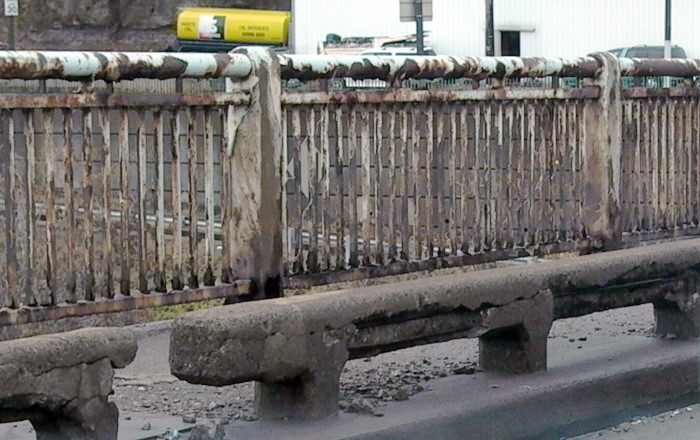
\includegraphics[width=0.65\linewidth]{roadway-splash.jpg}
  \caption{Effect of roadway splash on coated railing}
  \label{fig:roadway-splash}
\end{figure}

\subsubsection{Exposed Steel Bearings}
Steel bearings are often sheltered and isolated from water or salt water by the steel and roadway deck directly
above as shown in \cref{fig:bearing-difficult-protect}. On some structures, steel bearings can be the target of corrosion. At times bridges
must be closed to traffic and entire bearings must be replaced, which can require extensive shoring as shown in
\cref{fig:bearing-replacement}. Steel bearings can be exposed to an immersion-like environment as a result of leaks from joint areas
above.

\begin{figure}
  \begin{minipage}{0.3\linewidth}\centering
    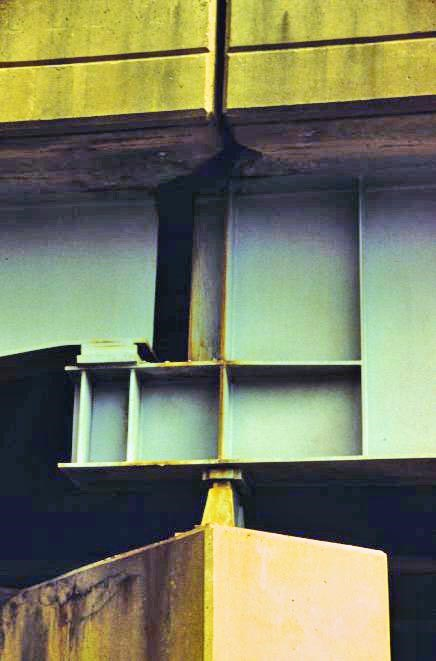
\includegraphics[height=4.5cm]{bearing-difficult-protect.jpg}
    % \caption{Bearings below roadway joints are difficult to protect (Courtesy KTA-Tator, Inc.)}
    \caption{道路下难以养护的支座}
    \label{fig:bearing-difficult-protect}
  \end{minipage}%
  \begin{minipage}{0.7\linewidth}
    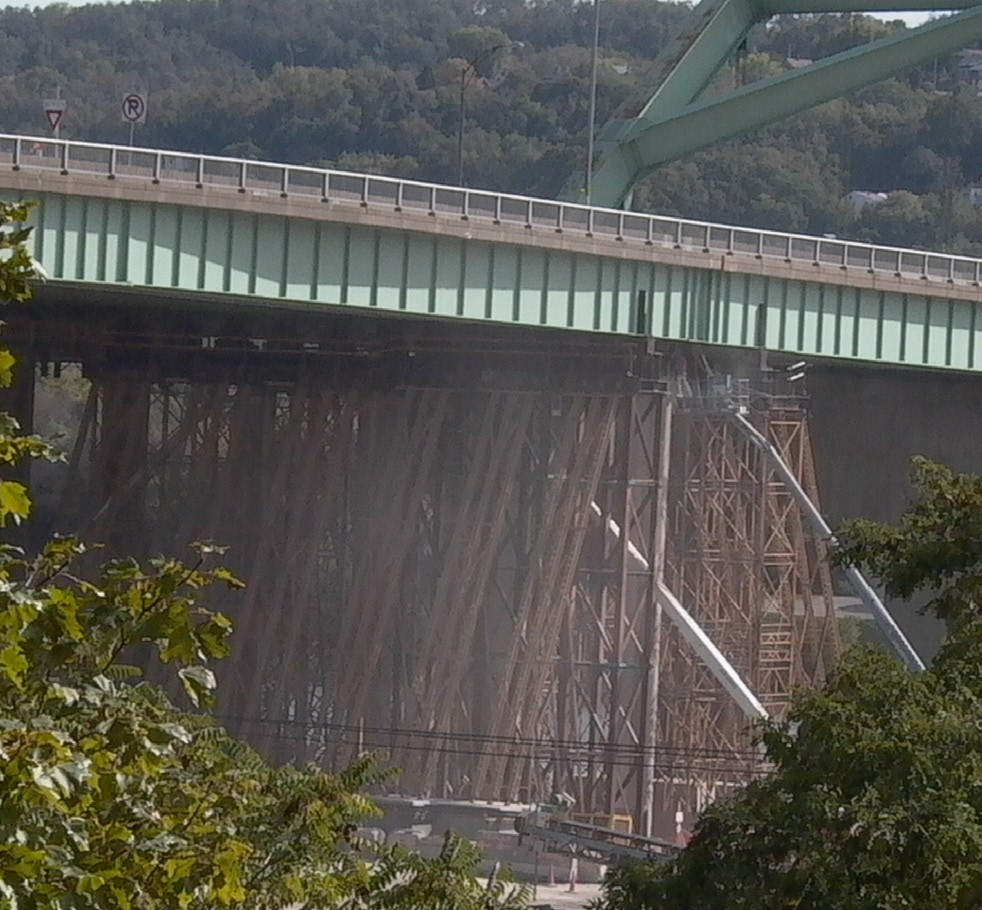
\includegraphics[height=4.5cm]{bearing-replacement1.jpg}\hfill
    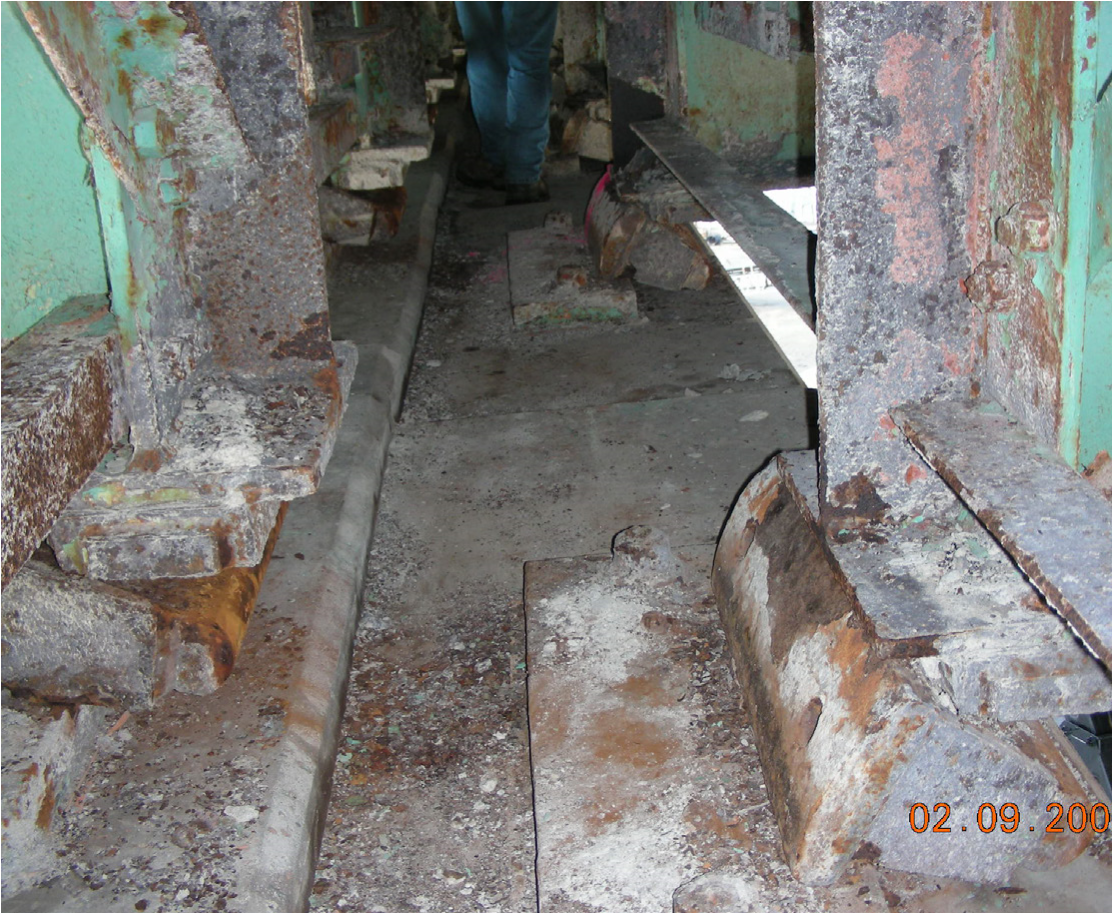
\includegraphics[height=4.5cm]{bearing-replacement2.png}
    % \caption{Shoring to support bridge during bearing replacement operation. Note heavy corrosion on bearings in the photo on the right.}
    \caption{支座更换期间支撑桥梁(注意右侧照片中支座严重腐蚀)}
    \label{fig:bearing-replacement}
  \end{minipage}
\end{figure}

\subsubsection{Back-to-Back Angles}
The use of back-to-back angles should be discontinued when new or replacement steel configurations are
encountered.

In rehabilitation maintenance, the use of back-to-back angles presents a configuration that is very difficult to
clean or coat effectively, and the use of great care in cleaning and coating such areas is recommended. Special tools,
often developed by the contractor for these special situations, are needed for effective protection and even then,
effective protection is usually unattainable.

\subsubsection{Wind Blown Rain or Salt Spray}
During rain, water can be blown onto steel surfaces even in those instances where there is a bridge sidewalk
above. The ability of a coating to withstand this occasional exposure to fresh, non-brackish water should not present
a problem for zinc-rich based coating systems.

On the other hand, storms can provide a benefit in that rain water can cleanse exposed surfaces. During storms,
salt water from nearby brackish water or from ice- or snow-melt can be blown by storms onto steel surfaces.
Repeated exposure to salt water is very corrosive, and the time of wetness and the number and length of wet/dry cycles affects the degree and extent of corrosion. In areas with a high time-of-wetness, for example frequent wet/dry
cycles, HDG or zinc spray metalizing should be considered for primary corrosion protection.

\subsubsection{Chlorides}
In a landmark literature survey compiled by Albias, von Loden, Onderzock and Advies, which was published in
the Journal of Protective Coatings and Linings (JPCL) in February, 1997, the researchers stated that “It has been
clearly established that soluble salts on the surface of steel will increase the rate of corrosion and paint breakdown for
many [coating] systems now in use.” This conclusion is as true in 2012 as it was in 1997. The authors offered
several conclusions:

\begin{itemize}
  \item From available data, it is not possible to establish a definitive allowable level of chloride contaminants.
  \item In relation to the durability of the paint system, a maximum chloride level of 10 to \qty{50}{\micro g/cm^2} is thought to be permissible, depending on the use and exposure conditions. This is only a rough guideline.
  \item Under specific conditions, higher maximum levels of chloride (up to hundreds of \unit{\micro g/cm^2}) are allowed for special, durable paint systems (e.g., zinc silicate).
  \item Exposure to marine conditions and/or industrial environments considerably increases the chloride contamination on steel.
  \item Abrasive blast cleaning does not remove all the chloride.
  \item Results of detection methods for soluble chlorides are affected by temperature, mechanical forces and the chemicals and type of analytical method used.
  \item The effect on steel of the hydrochloric acid generated as a consequence of the corrosion reaction is notable. Therefore, the removal of as much chloride as possible during blast cleaning and other surface preparation efforts is crucial. While there is still not complete agreement as to the precise level of chloride residue that is acceptable, SSPC-SP COM “ Surface Preparation Commentary for Steel and Concrete Surfaces”(2009), Subsection 4.3.6 “Soluble Salts” identifies three levels of chloride removal:
  \begin{itemize}
    \item \qty{0}{\micro g/cm^2}
    \item $< \qty{7}{\micro g/cm^2}$
    \item $< \qty{50}{\micro g/cm^2}$
  \end{itemize}
  \item A level commonly specified for conventional mild steel is \qty{7}{\micro g/cm^2}.
\end{itemize}

An FHWA-sponsored study by Appleman in 1995 concluded that the maximum safe level of chloride to remain when cleaning weathering steel was \qty{50}{\micro g/cm^2}.

In accordance with SSPC-SP 10, abrasive blast cleaning on non-corroded areas will reduce chloride levels to an acceptable $< \qty{7}{\micro g/cm^2}$. It will not always do so on heavily rusted, rust scale covered, or pitted or pack rust affected areas.

In some areas, it is believed that complete removal of all chlorides via only dry abrasive blast cleaning is at best
unlikely, and at worst, provides a false sense of security, even if white metal blast cleaning (SSPC-SP 5, White
Metal Blast Cleaning) is specified. Cleaning efforts beyond abrasive blast cleaning are usually needed. The use of
high-pressure water cleaning (HP WC), 5,000 to 10,000 psi, has been found to significantly reduce residual chlorides
to a very low level. High-pressure waterjetting (HP WJ), 10,000 to 30,000 psi, has also been used to reduce residual
chloride levels. As noted, the effect of chlorides on the corrosion rate of steel has been studied and well documented.

% \subsection{Factors Affecting Service Life of Galvanized/Painted Steel Bridge Elements Specific to a Galvanizing Coating}
\subsection{影响特定于镀锌层的镀锌/涂漆钢桥\glsentrytext{element}使用寿命的因素}
The corrosion protection of unpainted galvanizing comes from the formation of a thin, invisible layer of
insoluble corrosion products. Zinc, as an active metal, reacts with oxygen in the air, and zinc oxide starts forming
within about 24 to 48 hours after galvanizing and takes about a year for the zinc oxide to cover the entire galvanized
surface. The zinc oxide converts to zinc hydroxide upon exposure to moisture in the form of rain, dew, or high
humidity. The final step is the reaction of zinc oxide and zinc hydroxide with carbon dioxide in the air to form zinc
carbonate. This reaction requires free-flowing air. Zinc carbonate is the dense insoluble material that forms the
protective layer, sometimes called the patina. Zinc oxide and zinc hydroxide are water-soluble and not very dense.
They adhere loosely to the surface, so painting over zinc oxide or zinc hydroxide does not provide good adhesion of
the coating to the surface. The practical problem is that zinc oxide, zinc hydroxide, and zinc carbonate are all white
and cause the galvanized surface to appear a dull, matte grey, allowing no way to visually determine what form of zinc compound is present. Knowing the compound is important because some forms are not corrosion resistant and
are unsuitable for painting over.

\subsubsection{Reactivity of Zinc}
The reactivity of zinc is well-known to galvanizers. For instance, they know that if pieces are closely stacked
together for shipment, there will be no access to carbon dioxide in free-flowing air to form the zinc carbonate. In
such a case, only loose zinc oxide and zinc hydroxide will form, causing rapid consumption of the zinc. For this
reason, closely-spaced galvanized pieces should be unpacked. Upon doing so, the loose white deposit on the surface
should be noted. If this reaction process is allowed to continue, it can totally consume all of the zinc by reaction with
the moisture caught between the pieces. While rare, rusting of the unprotected steel may then occur, resulting in the
presence of rust beneath the deposit.

\subsubsection{Prevention/Passivation of White Storage Stain}
This white deposit is called "wet storage stain." Galvanizers apply a light coating of oil to prevent the stain. The
oil forms a barrier to keep moisture from reaching the zinc, thus preventing the zinc from being converted to oxide
and hydroxide forms. However, as paints do not stick to oil, painting the surface without first removing the oil is
unacceptable. This is true no matter what type of coating is applied. Another process used to prevent wet storage
stain is quenching or passivating with chromates or phosphates. Quenching (i.e., cooling and water bath) is not
harmful in and of itself. However the quenching bath may contain small amounts of oil and grease on the surface of
the water that are picked up when pieces are removed. Coatings also do not stick to chromate-quenched galvanizing,
but the phosphate improves adhesion. While wet storage stain can damage galvanizing, the methods used to prevent
it can affect painting results. It is always recommended to consult the galvanizers as to the process employed,
especially if the galvanized items are to be painted.

\subsubsection{Repair of Defects in the Galvanized Surface}
The next step in surface preparation is to repair any defects or handling damage. Galvanizing can leave high
spots and zinc droplets, which occur when a galvanized piece is withdrawn from the bath and excess zinc runs down
the edges onto a protrusion or irregular edge. Droplets form at edges where zinc drains from the piece and can be
removed with hand tools. High spots are usually ground down with power tools. Care is required to avoid removing so much zinc that the remaining thickness is below the specified minimum. SSPC-Guide 14, Guide for Repair of
Imperfections in Galvanized or Inorganic Zinc-Rich Coated Steel Using Organic Zinc Rich Coating, (2004) should
be consulted.

Unstable zinc oxide or zinc hydroxide may not have been entirely removed during the initial cleaning process.
There is no simple method for identifying the presence of either, so the surface must be further treated.

Galvanizing can be eroded if exposed to very strong acids or alkali, which may cause the zinc to dissolve as
metallic zinc is soluble in very strong acid or alkali environments. In these unusual circumstances, if re-galvanizing is
not possible, repairs can be made with coatings in accordance with SSPC-Guide 14 described above. After restoring
the zinc protection, a decision can be made as to whether painting is desired.


\subsubsection{Preparing Weathered Galvanizing for Painting}
Fully weathered galvanizing (i.e., galvanizing that has been outdoors for at least one year and preferably about
two) should have a fully-formed layer of protective zinc carbonate. Nothing is required to prepare the surface for
normal atmospheric exposure and its service life will not be limited in the normal course of exposure events. Bare
galvanized surfaces will be subjected to the vicissitudes of the local weather environment and this unknown, complex
exposure may mean that it makes sense to combine galvanizing and painting. A so-called duplex system (i.e.,
galvanizing and paint) should be considered. Such systems are said to provide 1.5 to 2.5 times the service life of the
sum of both galvanize and paint if each is considered separately, and an aesthetically-pleasing palette of colors is
available.

If a surface of weathered galvanizing is to be painted, the surface must normally be power washed with clean
water at about 1450 psi. Spot repairs of any damage in accordance with SSPC-Guide 14 are all that is necessary.


\subsubsection{Surface Preparation of New Galvanizing for Painting}
The often-made statement that galvanized surfaces “…cannot be painted” is incorrect. In fact, galvanized
surfaces are routinely painted successfully. The following are several steps in which errors of omission or
commission are routinely made, with remedies for each. There is no reason why so-called duplex systems cannot
perform for decades.

New galvanizing means galvanized steel that is between one or two days new and up to about two years old.

Wet storage stain, if present, must be removed before surface preparation. This can be done by brushing the stain
with a 1-2\% ammonia solution such as diluted household ammonia. After treatment, ammonia should be removed by
rinsing with warm water.

The first step in the surface preparation is to wash off oil, grease, and dirt. This is performed in accordance with
SSPC-SP 1 “Solvent Cleaning.” Water-based emulsifiers or alkaline cleaners work best. A mildly alkaline cleaner
should be used. The cleaning solution should be applied by dipping, spraying, or brushing with soft bristle brushes. A
temperature range of 140°F to 185°F works well. Afterwards, the surface should be thoroughly rinsed with hot water
and allowed to dry. One helpful tip for determining if oil was applied to the galvanized surface to prevent wet storage
stain is to contact the galvanizer; another way is to perform a water bead test in which a drop of water is placed on
the surface. If it beads, oil will probably be present. The best advice is that when in doubt, the entire surface should
be washed as described above. After the surface is washed, it should be examined for zinc ash, a residue that consists
of particles of oxidized zinc that float on the surface of the galvanizing bath. The ash can be removed by washing the
surface with a 1\% to 2\% ammonia solution.

Common methods for treating the surface in the field prior to painting are phosphating by the use of wash
primers, or sweep blast cleaning.

\paragraph{Phosphating Preparatory to Painting}
Phosphating is often accomplished by using a wash primer, a coating that neutralizes the surface oxides or
hydroxides and etches the galvanized surface. The most common wash primer is polyvinyl butyral, for example
SSPC-Paint 27. These materials are very thinly applied (0.3-0.5 mils) by brush or spray. The galvanized surface
should shadow through the coating at this thickness. If the galvanized surface is completely hidden, the wash primer
is too thick. Wash primers have poor cohesive strength and will split apart if they are too thick, resulting in paint
disbondment.

Phosphating is not recommended if a zinc-rich primer is going to be applied. Zinc-rich primers require intimate
contact between the zinc particles in the paint and the zinc metal on the galvanized surface. The zinc phosphate acts
as an insulator in the same way that iron oxide (i.e. rust) acts as an insulator on steel surfaces.

\paragraph{Sweep Blast Cleaning Preparatory to Painting}
Sweep blasting is a method of lightly blast cleaning that can remove zinc oxides on the surface and roughen the
surface without significantly removing the galvanizing. Sweep blast cleaning should be performed with abrasives that
are softer than the galvanized surface. The use of materials within Mohs scale hardness of five or less is suitable.
Sweep blast cleaning should be performed in accordance with SSPC-SP 7 “Brush-Off Blast Cleaning.”


\subsection{Factors Affecting Service Life of Steel Bridge Elements, Specific to Metalizing Coating}
Metalized coatings provide corrosion protection to steel by both sacrificial and barrier protection. The coating
itself provides a barrier between the environment and the steel surface, especially when applied in combination with
conventional sealer coatings (e.g., epoxies, polyurethanes, acrylics, etc.) as topcoats. Due to the electrochemical
reaction between steel and zinc or aluminum in an aqueous or salt-contaminated environment, these coatings
sacrifice themselves to protect the steel at the site of any damage, or holes, in the coating. This sacrificial protection
is akin to the protection provided by zinc-rich primers or galvanizing.

\subsubsection{Metalized Coatings}
Metalized coatings can be applied in the shop or in the field using a variety of techniques and equipment. The
metal or metal alloy is applied in wire form and is fed through a source and liquefied. The source may be either
flame (i.e., oxygen-acetylene) or electric arc. The liquefied metal is immediately propelled onto the prepared steel
surface using airspray in a manner similar to that used in painting. Once on the surface, the liquid metal cools and
dries very quickly to form a continuous protective coating over the steel surface.

\subsubsection{Cost of Metalizing}
Recent (2012) cost estimates place metalizing as 2 to 3 times per square ft. the cost of conventional painting. A
recent project at a large fabricator queried indicates that a significant differential currently exists. On a best-case
basis, it is estimated that metalizing costs at least 40\% to 50\% more than painting.

\subsubsection{Salt-Contaminated Areas}
Metalized coatings consist of spray droplets which have solidified and overlapped providing a somewhat coarse
matrix. This matrix is a barrier coating as well as a chemically active one due to the anode/cathode relationship
between zinc and iron. The primary benefit of metalizing over other coating technologies is its durability and corrosion resistance especially in salt-rich environments. For this reason, the application of metalizing should be
considered as an option for bridge structures in salt-rich environments or for areas or components of bridge structures
which receive considerable exposure to salt and moisture from drainage and runoff. While there are cost differences
between metalizing and painting, in many cases metalizing should be specified. Based on the performance of
metalizing over a long period of time, repairs and renovations on steel bridges would benefit by its use.

Metalized coatings have been shown to perform very well in studies when applied over steel that has been blastcleaned
in accordance with SSPC-SP 5, “White Metal Blast Cleaning,” or SSPC-SP 10, “Near-White Blast
Cleaning.” These coatings have a dull, grey appearance with a rough texture as applied, but may be sealed and
topcoated with most conventional paints. Sealing is recommended by many existing guidelines as it tends to increase
coating life, reduce the deleterious effects of metalized coating porosity, and improve aesthetics 

Metalized coatings provide the benefit of defect tolerance. The sacrificial nature of these coatings provides
corrosion protection to the underlying steel at the site of breaches in the coating film. Metalized coatings, particularly
aluminum and aluminum alloys, also tend to be quite abrasion resistant.

\subsubsection{Bond Strength}
The bond between the metalized coating and the steel surface is mechanical in nature. As such, the bond is
sensitive to surface contaminants and to the shape of the surface profile. Surface preparation should be specified as
above (SSPC-SP 10 or SSPC-SP 5 with an angular 2-4 mil anchor (tooth) profile).

Blast cleaning with rounded steel shot has produced deficient adhesion results and as such steel shot abrasives
should not be used on surfaces which will or may be metalized.

As a "solventless" coating application method, metalizing is less forgiving than conventional paint application.
Applicators must be properly trained and experienced with the specific equipment and metals or alloys to be used.

Because metalized coatings are inherently porous, achieving an adequate coating thickness (6-8 mils min.) in an
overlapping spray pattern is critical to coating life.

\subsubsection{Field vs. Shop Application}
Metalizing technology may also be applicable to field maintenance coating operations where a long-term,
durable corrosion protection coating system is required. Applications of metalized coatings in the shop, and
particularly in the field require technically sound specifications and practices.

\subsection{Factors Affecting Service Life of Steel Bridge Elements, Specific to Weathering and Noncorrosive Steels}

\subsubsection{Corrosion Resistant Weathering Steel}
With the introduction of steel as a material of construction for bridges in the late 1800s, the industry has sought
to find a form of steel that can overcome its most basic limitations—corrosion. It was believed that an answer had
been found in the 1970s with the introduction of weathering steel. Since the 1970s, the search for the ideal material
has evolved through improved higher strength weathering steel—high performance steel (HPS). Each step has
produced incremental improvements in the performance of weathering steel in a normal weathering environment.
Unfortunately, there has been even wider application of the use of weathering steel in bridges at locations which are
not recommended for the best use of weathering steel. These areas are often in heavily salted areas, or are in areas
where the steel is sheltered or exposed to other conditions in which the very corrosion-resistant patina simply does
not form. These areas are discussed elsewhere in this chapter.


\subsubsection{A1010 Structural Stainless Steel}
Although initial corrosion studies performed on A1010 steel have been very favorable, the use of A1010 steel is
currently inhibited somewhat by its premium cost. It is believed that with sufficient production, volume costs will
come down. While testing has produced promising results, its performance in aggressive, salt-laden areas is not
completely known. Even with these unknowns, however, it is hopeful that a solution to the 125+ year-old problem of
dealing with the corrosion characteristics of steel will be determined. As additional bridges are constructed using
A1010 steel, time will tell. Currently (2012), one bridge has been completed in California and two others are under
construction in Oregon.

% \section{Options for Enhancing Service Life with Respect to Corrosion Performance of Steel}
\section{钢的抗腐蚀性能方面提高使用寿命的选择}

\subsection{General Categories of Solutions for Preventing Corrosion of Steel Bridge Elements}
\label{subsec:category-solution-prevent-corrosion-steel}
In general, there are three options for developing corrosion prevention systems for steel bridges:
\begin{enumerate}
  \item The use of a coating system, which can consist of paint, galvanizing, or metalizing systems;
  \item The use of corrosion resistant steel (weathering steel) or non-corrosive steel; and
  \item Avoidance of corrosive environments or corrosion-prone details.
\end{enumerate}
\subsection{General Strategies Capable of Producing Effective Corrosion Protection System}
Regardless of the option selected from the list provided in \cref{subsec:category-solution-prevent-corrosion-steel}, there are five major strategies that can result in an effective corrosion protection system. These are described in the following sections.
\begin{itemize}
  \item Design review to assure that the best protection is designed into the structure,
  \item Use composite protection,
  \item Use corrosion-proof materials
  \item Employ super-durable coatings, and
  \item Use on-going engineered maintenance painting.
\end{itemize}
\subsubsection{Designing Corrosion Protection into the Structure from the Beginning}
Through the first 125 years of the steel bridge era, steel bridges have benefitted from the corrosion control
foresight utilized by their designers. The elimination or minimization of corrosion on such structures has resulted in a
knowledge base which, if systematically applied to every structure, can benefit each one. As these lessons-learned are
applied, the corrosion resistance features, principles, experiences, and insights should be designed into every new and
rehabilitated steel bridge. Actions taken during the earliest project design stages can cause a dramatic lengthening of
the coatings part of the maintenance/repair/replace cycle by the elimination of areas likely to corrode early in the
service life of a structure. It is known that if corrosion resistance is designed into a structure, by carefully managing
the configuration and details of bridge design and detailing, while using the current coatings systems, bridge
corrosion resistance should improve dramatically. This design review should be considered a design hold-point. In this instance, hold point means that further progress on the design would depend on having a corrosion review
performed and a corrosion resistance control plan initiated.

This design phase review is a major means for creating a 100-year life for a new steel bridge. In order to attain
100 years of service life, it will be necessary to develop and utilize preferred details, which will serve as a way to
lengthen the time before any maintenance painting is needed during the structure’s expected 100-year service life.

\begin{figure}
  \begin{minipage}{0.4\linewidth}\centering
    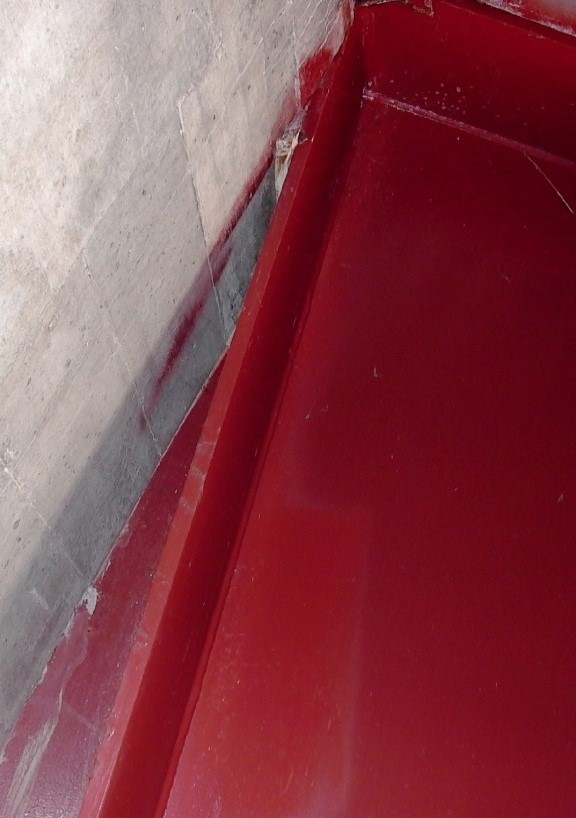
\includegraphics[height=5.5cm]{details-difficult-paint1.jpg}
    % \subcaption{Lack of stiffener clearance to back wall results in an almost  unpaintable detail.}
    \subcaption{与背墙间缺乏涂装作业空间的构造}
  \end{minipage}
  \begin{minipage}{0.4\linewidth}\centering
    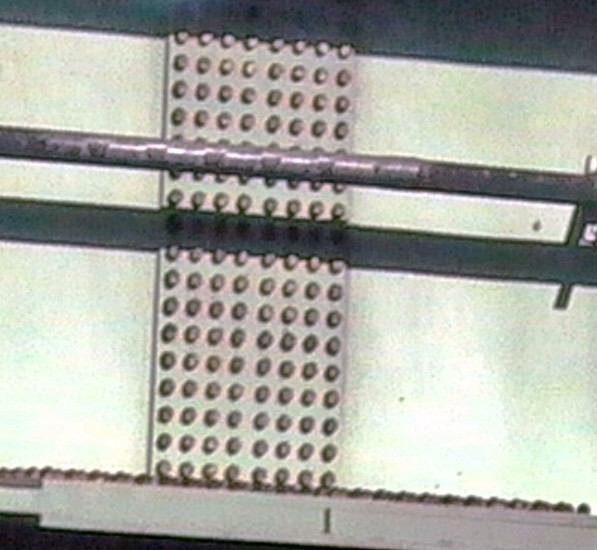
\includegraphics[height=5.5cm]{details-difficult-paint2.jpg}
    % \subcaption{Coating failure at splice, especially around fasteners.}
    \subcaption{接头处尤其是紧固件周围无法进行涂装}
  \end{minipage}
  % \caption{Details difficult to paint}
  \caption{难以进行涂装的细部构造}
  \label{fig:details-difficult-paint}
\end{figure}

\subsubsection{Composite Protection}
\label{subsubsec:composite-protection}
Currently the use of zinc to protect steel from corrosion is the gold standard of care. The use of a composite
protection strategy is based on the premise that there is an order of efficacy in terms of corrosion protection provided
by zinc as delivered in its various forms.

Hot-Dip Galvanizing (HDG) is considered the most efficacious protection because of the iron/zinc alloy that is
formed on the steel surface closest to the outside of the HDG part. Thereafter, even if the HDG surface is nicked, the
alloy layer will afford substantial protection from corrosion. Many smaller bridge elements, steel bearings, cross
frames, bolts, and expansion devices, etc. can be protected with HDG.

Metalizing, as noted, has been tested for decades and also found to be excellent means of protecting steel from
corrosion. The spray–applied zinc does not form an alloy layer like HDG, but does provide zinc in intimate contact
with steel (iron) in order to provide effective galvanic protection. Metalizing has been tested repeatedly in both the
laboratory and field and found to provide a very high level of corrosive protection.

Zinc-rich, primer-based coatings systems have been the workhorse of the steel bridge industry for over 40 years
and coatings systems based on zinc-rich coatings have a successful track record on countless bridges.

Uncoated weathering steel also has a 40-plus year history of providing successful corrosion protection in certain
exposure areas.

Structures and parts of structures can be protected using combinations of protective steps, for example steel
bearings or cross frames can be hot-dip galvanized or metalized and then painted. Some fasteners (ASTM A-325
bolts) are available with either an HDG or mechanically-galvanized coating and either can be coated or not as
required.

A composite approach is often adopted on weathering steel bridges when girder ends are cleaned and coated.

\begin{figure}
  \begin{minipage}{0.55\linewidth}\centering
    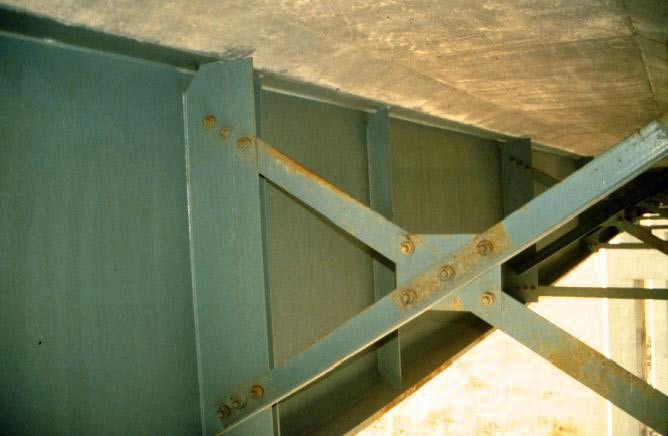
\includegraphics[height=5cm]{detail-composite-protection1.jpg}
    % \subcaption{Welded cross frame could be galvanized.}
    \subcaption{焊接十字框架可以镀锌}
  \end{minipage}%
  \begin{minipage}{0.45\linewidth}\centering
    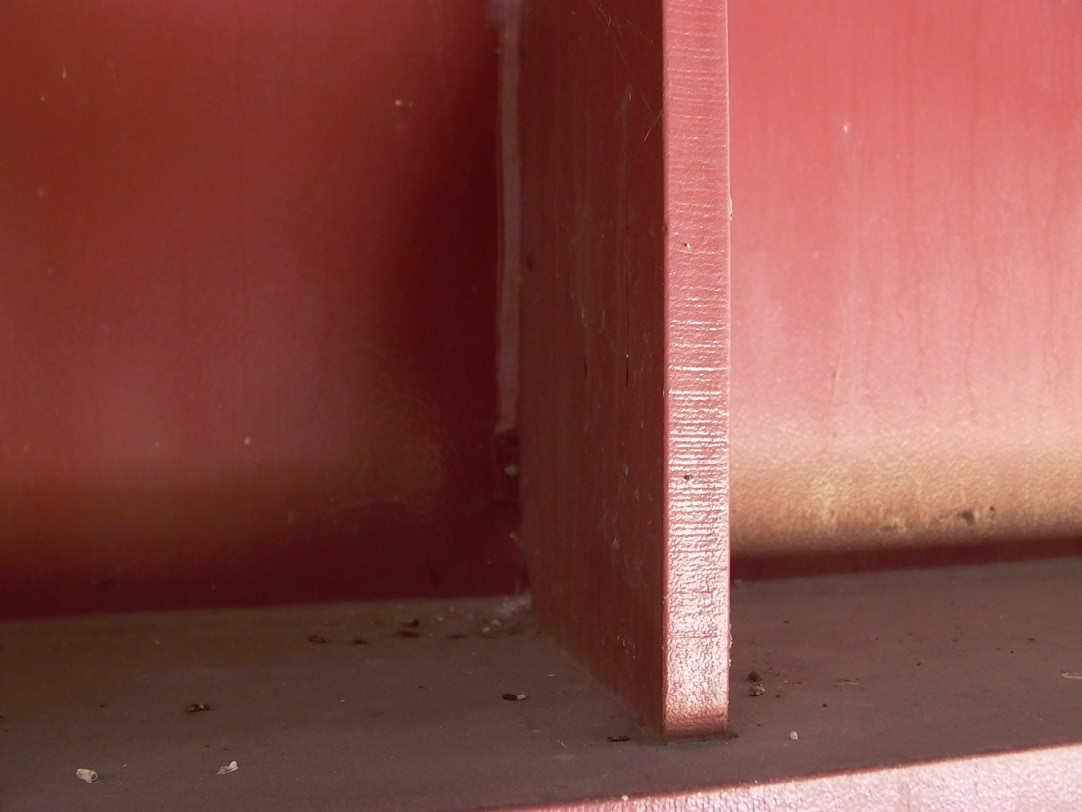
\includegraphics[height=5cm]{detail-composite-protection2.jpg}
    % \subcaption{Mill to bear stiffener leaves crack in the coating design}
    \subcaption{磨机承受加强筋在涂层设计中留下裂纹}
  \end{minipage}
  \begin{minipage}{\linewidth}\centering
    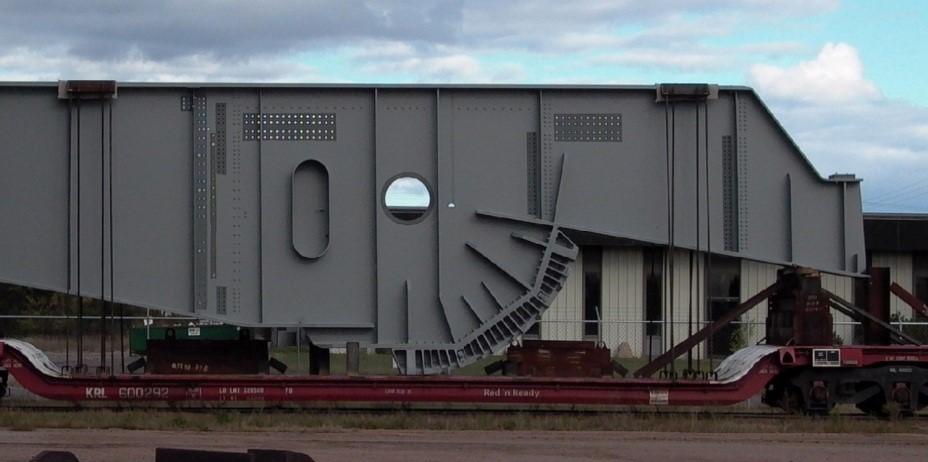
\includegraphics[width=0.75\linewidth]{detail-composite-protection3.jpg}
    % \subcaption{Large trunnion girder for a lift bridge-a unique opportunity for composite protection is presented by its configuration.}
    \subcaption{用于升降桥的大耳轴梁——其配置提供了一个独特的复合保护机会}
  \end{minipage}%
  % \caption{Details suitable for composite protection. (All photos courtesy KTA-Tator, Inc.)}
  \caption{适合复合保护的细部构造}
  \label{fig:detail-composite-protection}
\end{figure}

In the future, ASTM A1010 or a similar material may conceivably be routinely employed in coastal areas or
where salt usage is a certainty. It may prove feasible to utilize A1010 in combination with weathering steel. In such a
case, perhaps girder ends could be made of A1010 steel, while the remainder of the girder is comprised of weathering
steel or painted regular mild steel.

\cref{tab:apply-zinc-to-steel} is a summary of the comparative functionality of galvanizing/metalizing and zinc-rich paint in terms of
cost, protection, and durability.

\begin{table}
  % \caption{Three Ways to Apply Zinc to Steel. (KTA-Tator, Inc.)}
  \caption{将锌应用于钢材的三种方法}
  \label{tab:apply-zinc-to-steel}
  % \input{tables/apply-zinc-to-steel}
\end{table}

In the table, the heading term “Duplexable” refers to the particular coating’s ability to be combined with other
types to provide a composite coating system. In the column, the term Y signifies yes, G represents Galvanize, M
represents Metalize, and P represents a paint layer. For example, galvanizing can be combined with a top paint coat,
and zinc-rich paint as a primer can be combined with multiple additional paint layers

\subsubsection{Use of Corrosion-Resistant or Corrosion-Proof Materials}

\paragraph{Corrosion-Resistant Steel}
Weathering steel (coated or uncoated) has been the subject of much research and discussion since its initial use
on bridges in about 1970. Weathering steel’s roots lay in the improvement in the corrosion resistance of steel when
small amounts of copper, chromium, nickel, phosphorous, silicon, manganese, or combinations thereof, are added to
carbon steel. When weathering steel is properly exposed, a rusty red-orange to brown or purple-tinted patina forms.
When the patina is formed, the corrosion rate of the steel stabilizes within about three to five years. The formation of
the protective patina requires a series of wet and dry periods. In certain situations, the protective patina does not form
completely or not at all. For example, when the steel is sheltered from the rain, the dark patina cannot form. In areas
with high concentrations of corrosive industrial or chemical fumes, weathering steel may exhibit a much higher
corrosion rate. In a saltwater marine environment or in areas heavily exposed to chloride-containing deicing
materials, the protective patina does not form. The use of uncoated weathering steel in such locations is not
recommended.

When weathering steel is used in locations where regular wet/dry cycles occur, the steel is corrosion resistant to
the point that no coating is necessary. In some locations, weathering steel enjoys vastly enhanced corrosion resistance
which can render it relatively impervious to corrosion. The exact degree of corrosion resistance afforded is dependent
upon a number of variables, including climatic conditions, pollution levels, and the degree of sheltering from the
atmosphere, as well as the composition of the steel itself. These variables influence the areas in which the use of
weathering steel is appropriate.

In a survey conducted as a part of the SHRP 2 R19A Project (final report forthcoming), about one third of the 16
DOTs responding reported the use of weathering steel on over 50\% of their steel bridges.

Many states use the guidance document published by the Federal Highway Administration, FHWA T5140.22
Technical Advisory, Uncoated Weathering Steel in Structures (FHWA 1989). Note that the Technical Advisory for
weathering steel use is in the process (as of 2012) of being revised and updated by the FHWA.

In order to shield the weathering steel in areas likely to experience chloride-laden water exposure, many states
paint the end of the weathering steel members for a distance of 1.5 to 2 times the depth of the web. The same zincrich,
primer-based coating systems used by the various DOTs for non-weathering steel are employed. In other locations, weathering steel is used for its other characteristics and is coated in its entirety for protective and/or
aesthetic reasons.

\paragraph{Non-Corrosive Steel}
The “perfect” weathering steel would be a material that is corrosion proof in all environmental conditions. Such a
material would present a desirable solution to addressing the main limitation of steel as a construction material, that
is to say, steel, rusts. And steel rusts even more in the presence of chlorides. Therefore, the “perfect” material would
be a true “unpainted, corrosion resistant solution” for any environment.

A steel product believed by some to meet these stringent requirements has now been developed. The corrosion
resistance has been accomplished by chemically augmenting the steel’s metallurgical composition. This new grade of
weathering steel, ASTM A1010, contains 10.5\% to 12.5\% chromium and is said by its vendors to be immune to
corrosion based on testing performed in Kure Beach, NC in the 25-meter test site. (See Figure 6.18.)

This “corrosion proof” steel is just beginning to be used on bridges. One small structure was constructed in 2004
in Colusa County, California. This project was the subject of a report presented at the 2004 Prefabricated Bridge
Elements and Systems Conference. The bridge design was a prefabricated lightweight section referred to as a multi--
cell box girder (MCBG). Less than 23 tons of A1010 were needed to form the structure of this short span bridge
with overall dimensions of 72 ft long by 32 ft wide.

Construction of two bridges using A1010 steel is underway in Oregon, and the possibility of constructing other
bridges has been mentioned in other states.

Although A1010 steel remains a somewhat costly alternate material choice, it does demonstrate that it may be
possible to anticipate the use of such a material in the future.

\begin{figure}
  % \includegraphics[width=\linewidth]{graphic-file}
  \caption{Corrosion resistance of A36, A50W, HPS 70W, 100W and A1010 grades of steel exposed at Kure Beach, North Carolina. (Fletcher et al., 2003)}
  \label{fig:corrosion-resistance-a36et}
\end{figure}

\subsubsection{Use of Super-Durable Coatings}
The search for the “Superman” of coatings continues:
\begin{itemize}
  \item FHWA has an active coatings RD\&T Program, which recently has focused research on two-coat systems and
  their ability to perform as well as the traditional three-coat system that has been in use since around1965.
  Testing of one-coat system candidate materials for steel bridges has also been underway. FHWA has released
  its final report on that testing as FHWA Report HRT11-046 in June. 2011. While there were some promising
  prospects among the materials tested, none of them approached the performance of the three-coat control
  system in the testing.
  \item On-going efforts to identify new resins and pigments for improved coatings are underway in the private
  sector.
  \item Developing new super-durable coating materials via both basic and applied research efforts, including
  industry-to-industry technology transfer, is underway. The use of nano particles in coatings has begun but has not yet spread to the bridge industry. The potential use of nano-sized (a billionth of an in.) pigment
  particles that can dramatically alter the performance of a coating is much anticipated.
  \item In new construction, the coating systems and procedures are basically unchanged since the late 1960s. For
  new bridges the steel is coated using a system consisting of a zinc-rich primer, usually an epoxy mid-coat
  and usually a urethane topcoat, applied over steel cleaned in accordance with SSPC-SP 10 Near-White Metal
  Blast Cleaning. Initial cleaning and priming is normally done in the fabrication shop.
\end{itemize}

\subsubsection{Maintenance Painting}
As in many other areas of the construction industry, quality in bridge painting must be built-in and cannot simply
be added after the fact. Properly selected and applied coatings can often last for many decades with periodic planned
maintenance painting. A comprehensive approach to maintenance painting requires considerations of surface
preparations, inspection, and proper planning.

\paragraph{Surface Preparation}
The initial condition of the surface to be cleaned will determine the amount of work, time, and money required to
achieve any particular degree of surface cleanliness. It is more difficult to remove contaminants from rusty steel and
to remove mill scale from new steel than it is to wash surface film off of steel in good condition. Therefore, it is
necessary to consider the surface condition prior to selecting the method of cleaning. The method of cleaning is an
integral part of how the coating system may be expected to perform in any given environment. The initial condition
of the steel may determine the choice of abrasives. Steel shot is an economical and effective choice for removing
intact mill scale. Although their use in the field is not unknown, steel abrasives are usually recycled and therefore
find their most common usage in the shop. However, if the steel is rusted or pitted, an angular abrasive, such a steel
grit or a non-metallic mineral abrasive, will more effectively scour out the rust.

The initial conditions encountered can be broadly divided into three categories as follows:
\begin{enumerate}
  \item New construction—steel not previously coated;
  \item Maintenance—repainting of previously coated, painted, metalized or galvanized steel; and
  \item Contaminated surfaces—common to both new construction and maintenance.
\end{enumerate}

Typical contaminants that should be removed during surface preparation are rust, corrosion products, mill scale,
grease, oil, dirt, dust, moisture, soluble salts (i.e., chlorides, sulfates, etc.), paint chalk, and loose, cracked, or peeling
paint. Discussions of each of these follow.

Rust, Rust Scale, and Pack Rust. Rust consists primarily of iron oxides, the corrosion products of steel.
Whether loose or relatively tightly adherent, rust must be removed for satisfactory coating performance. Rust
resulting from the corrosion of steel is not a good base for applying coatings because it expands and becomes porous.

Ideally, rust and rust scale should be removed, even when using the lowest degrees of hand and power tool
cleaning (SSPC-SP 2, Hand Tool Cleaning, and SSPC-SP 3, Power Tool Cleaning). Judgment should be used on an
individual project basis whether the cost and effort required to remove the stratified rust, rust scale, and to a greater
or lesser extent, pack rust, can be justified by the expected increase in the life of the coating system.

To effectively repair pack-rusted joints, it may be necessary to remove rivets, separate the plies of steel, clean,
paint, and refasten with bolts.

On riveted and bolted connections, bridge management practices are required that cause surfaces to be repaired
long before such inefficient, costly repairs are necessary. It is obvious that many square feet of steel can be cleaned
and recoated before the cost of disassembly and reassembly of bridge connections is equaled.

The existence and treatment of rust and particularly pack rust can make bridge repair so expensive that bridge
demolition may appear to be a feasible option. When such matters are expected to be at issue, agreement about the
extent of removal of these materials should be reached prior to the start of work.

There is a trade-off between repair cost and extended service life. For maintenance repainting, the degree of
surface preparation required depends on the new coating system and on the extent of degradation of the surface to be
painted. The amount of rusting on the surface is based on the numerical scale of zero to 10, given in SSPC-VIS 2,
Standard Method of Evaluating Degree of Rusting on Painted Steel Surfaces (2000), in which a reading of 10
indicates no rust and a rating of zero indicates more than 50\% rusting. SSPC-PA Guide 4, Guide to Maintenance
Repainting with Oil Base or Alkyd Painting Systems, (2004) suggests the minimum surface preparation needed for
each degree of rusting. This guide includes a description of accepted practices for re-cleaning old, sound paint,
removing rust, and feathering the edges of sound coating around the area and recoating. Additional information on the subject may be found in SSPC-SP COM, Surface Preparation Commentary for Steel and Concrete Surfaces
(2004).

\emph{Mill scale} is a bluish, normally slightly-shiny outside residue that forms on steel surfaces during hot rolling at the
steel mill. Although initially tightly adherent, it eventually cracks, pops and disbonds. As a general rule, unless it is
completely removed before painting, it will, at some point, most likely crack and cause the coatings to crack,
exposing the underlying steel surface. In addition, steel is anodic to mill scale and as the anode in the resultant
dissimilar metals corrosion cell (with oxygen from the air and moisture) will corrode more rapidly.

At least in the short term, mill scale is somewhat unpredictable in its effect upon the performance of coatings,
although, as noted, tightly adhered, intact mill scale may not have to be removed at all for steel exposed to a mild
atmospheric exposure. However, if the steel surface is to be coated with primers with low wetting properties, or
exposed to severe environments such as wetness or immersion in fresh or salt water, then removal of mill scale by
blast cleaning or power tool cleaning is necessary.

\emph{Soluble salts} are deposited from the atmosphere onto surfaces. If they are permitted to remain on the surface
after cleaning and are coated over, they can attract moisture that can delaminate the coating and cause blisters. Salts,
particularly chlorides, may also accelerate the corrosion reaction and underfilm corrosion. Methods for measuring
the amount of salt on the surface are described in SSPC-Guide 15, Field Methods for Retrieval and Analysis of
Soluble Salts on Steel or Other Nonporous Substrates (2005). In some circumstances, it is desirable to remove
soluble salts by power washing or other methods employing wet methods prior to power tool or abrasive blast
cleaning. In other circumstances, salt removal is more efficient after the member has initially been subjected to
abrasive blast cleaning.

The removal of this non-visual surface contaminant is an area in which extra effort in cleaning will help
immeasurably in improving coating durability.

\emph{Ultraviolet light degradation}. The sun’s ultraviolet light causes exposed organic coating to chalk to some
extent. Chalk is the residue left after deterioration of the coating’s organic binder on exposed surfaces. All loose
chalk must be removed before coating in order to avoid intercoat adhesion problems.

\emph{Sharp edges}, such as those which at times may occur on some rolled structural members or plates, as well as
those resulting from flame cutting, welding, grinding, and shearing, could have an influence on coating performance
and may need to be addressed.

Additional guidance on the subject of material anomalies and sharp edges can be found in AASHTO/NSBA Steel
Bridge Collaboration Specification S 8.1, Guide Specification for Application of Coating Systems with Zinc-Rich
Primers to Steel Bridges. (2006)

\paragraph{Coatings (Paint) Inspection}

The importance of coating inspection during surface preparation and coating application cannot be ignored or
under-emphasized.

As a general rule, it is not possible to visually examine a coated surface and know whether the surface
preparation and coating application was done in accordance with the applicable specification and good painting
practice. Determining whether the coating material was properly mixed; whether a component was substituted,
adulterated, or left out completely; or whether an entire coat of paint was simply skipped, can be a tedious, costly
process. Once a surface has been painted, it is usually not possible to determine whether each painter in a crew has
complied consistently with the specification. It is important to recognize the value of adequate inspection.

Unless trained inspectors monitor the entire operation from start to finish, there is no way to know for sure about
the level of specification compliance actually achieved; coatings systems can only perform if they are properly
installed.

Certification programs for bridge paint inspectors are offered by the Society for Protective Coatings. The SSPC
Bridge Coatings Inspector (BCI) training course was developed by a committee of more than a dozen DOT
representatives. The course is appropriate for any level of worker in the coatings industry including apprentices,
blasters, painters, foremen, superintendents, engineers, and inspectors. Details about the BCI course can be found at \url{www.sspc.org}.

Attendance at the BCI class is designed to instruct the attendees to be able to do the following:
\begin{enumerate}
  \item Define the varying professional rules of the inspector, bridge owner, and painting contractor and the relationship to each other at the project site;
  \item Identify what preparation the inspector must make prior to the start of work in order to conduct effective inspections;
  \item Recognize common coating inspection and related terms;
  \item Identify and properly adjust and operate commonly-used coating inspection instruments and test
  apparatus;
  \item Identify fundamental surface preparation and coating application processes;
  \item Identify key documents (e.g., specification, product data sheets, and technical bulletins; industry
  technical standards; and references) required to perform competent inspections;
  \item Identify inspection check or hold points;
  \item Create inspection documentation, including a basic inspection plan;
  \item Identify processes normally inspected and documented; and
  \item Identify common coating application defects
\end{enumerate}

There are a variety of other inspection training classes offered by private organizations and nonprofit societies.
While all have strengths, it is noted that the SSPC BCI trained and certified coatings inspectors have received
training prepared specifically for the coating of steel bridges. The SSPC-trained BCI is considered by many to be the
most experienced and best-trained bridge coating inspector in the bridge coatings inspection field, and many of
SSPC’s coatings inspection training courses include the preparation of inspection plans in the curriculum.

In order to provide both guidance to those responsible for creating quality control plans and a training document
for course participants, SSPC developed a Guide for Planning Coating Inspection in 2008. The planning guide
begins by describing the importance of quality monitoring on a project to reduce the risk of coating failure, and
describes the challenges associated with trying to assess quality after the project is complete. It also stresses the
importance of planning the inspection to increase the likelihood that inspections are performed and the results
properly documented. The intended purpose of the planning guide is to assist coating inspectors, quality control
personnel, and owners with the development of a tool to help ensure the coating or lining installation is the best it can
be.

\paragraph{Worst First Versus Engineered Maintenance Painting}

Many agencies are perennially short of maintenance painting funds. As a result, the bridges that receive coating
attention are those that appear to be in the most distress (worst-first). By the time a structure appears to need the
most attention, it is probably well past the point at which the spot-on zone cleaning can be effectively employed. The

SSPC Technology Update TU-3, Overcoating (2004), offers guidance when considering overcoating. In Appendix
A, Subsection A2, Painting Scenarios, Subsection A.2.1 entitled Bridge Painting Using Risk Tables deals with the
percent of the surface at which the cost of the repairs approached that of full removal. The percentage identified as
the critical percentage beyond which the surfaces are rusted or distressed such that surface preparation is necessary is
16+\% (per ASTM D610, Rust Grade 2. Note Rust Grade 10 = essentially no rust, while Rust Grade 0 = >50\% rust)
SSPC reports in this document that according to the AASHTO Guide for Painting Steel Structures, (AASHTO
1994) “whenever the surface preparation area exceeds 15\% to 20\% of the surface area, the economics are such that a
total removal of lead paint is the most viable option.”

As noted above, from a cost perspective, the difference in cost between spot or zone cleaning and painting versus
full removal is dramatic. According to industry sources, a typical lead paint removal project in the northeastern part
of the United States (in 2011) averages ~ \$13/sf. Of that amount, about half or \$6.50/sf is attributed to surface
preparation (access cost, containment, equipment, abrasive, and labor).

If spot or zone cleaning were possible, costs on a comparative basis would be about \$3.90 (30\%). If cleaning
were performed when the surface affected was >3\% (Rust Grade 4) but <10\%, costs would be lower still.

It is apparent that a timely touch-up would extend the service life of the paint project and lower costs. The
reasons for being forced into a “worst-first” mode vary, but the practice is common. If an engineered approach to
maintenance recoating were employed, overall costs could be reduced by a large percentage and the condition of the
coatings on the bridge inventory in a given city, district, or state would, in time, improve.

It is recognized that bridge maintenance activities are driven by many factors, not all of which are corrosion
related. When the matter of maintenance painting is considered, the utilization of an engineering approach will help
to counter the worst-first approach. If the de facto use of the worst first practice is unchanged, coatings costs will be
at their highest.

If every bridge which was repainted, even if completely re-done, were placed into a master schedule of planned
paint touch-up in say 20 years, eventually the worst bridges would be repainted and those structures which are able to
be recoated to extend their service lives would emerge as the norm. There are further enhancements to the planning
that can be employed. For example, the deterioration of one structure may be faster than another. In those cases, the
examination and evaluation of a structure can be scheduled in a different cycle.

Early intervention saves money; can stretch the budget to cover additional projects; and can eventually improve
the condition of the steel structures across an area, district, or even an entire state.


\subsubsection{Bridge Maintenance Owner’s Manual}

Every new bridge and every rehabilitated structure should be delivered with an owner’s manual containing a
lifetime maintenance plan which outlines, much like an automobile owner’s manual, when designated corrosion
mitigation activities are to be undertaken.

For example, it might be recommended that coating touch-up of minor nicks, scratches, etc. be undertaken every
five years and that every 25 or 30 years, whenever certain conditions exist, the structure be touched up and
overcoated. Following this maintenance plan based on known, needed activities, would allow the owner to achieve
the service life inherent in the structure.

\section{Strategy Selection Process}
There are a wide variety of coating systems among which a specifier can choose. Several of these systems are
recognized by the coatings industry as having a track record of successful performance in a given service
environment. These systems are assembled by the coating manufacturer according to product, Note that in many
cases, a given system can be used in a multitude of locations and service environments. For example, a zinc-rich
primer/epoxy intermediate coat/acrylic polyurethane topcoat can be used to protect bridge steel in most areas and has
a 40+ year service history.

A coating system is selected based on the prevailing service environment, the intended life of the structure, the
level or degree of surface preparation possible, the intended service life of the coating, access, and any other
constraints.

A chart listing common generic coating systems follows. It includes common service environments within a
given structure and coating systems candidates for each. Note that this chart represents a cross-section of coating
systems.

\begin{table}
  \caption{Coating Systems for Highway Bridges (New Construction and Maintenance). (KTA-Tator, Inc)}
  \label{tab:coating-system-highway-bridges}
  % \input{tables/coating-system-highway-bridges}
\end{table}

Maintenance overcoating is a process in which new coating is applied over existing coating. Based on industry
knowledge and DOT survey information obtained for this project, the coating systems currently in use for this
purpose include acrylic, calcium sulfonate, epoxy sealer/epoxy/urethane, epoxy sealer/urethane, polyester and
polyaspartic.

Maintenance recoating is a process in which a new coating system is applied over a surface from which all old
coating has been removed. According to the DOT survey information described above, the most commonly used
systems consist either of an organic or inorganic zinc-rich primer with an epoxy mid-coat and a urethane topcoat.

It is noted that these zinc-rich primer based systems have proven themselves in the field on thousands of
structures for over 40 years. In the bridge industry, few materials have this proven track record. No doubt the
demonstrated longevity of the systems has contributed to their continued use.

\subsection{Characteristics by Coating}
\cref{tab:coating-characteristics} is a chart listing common coating types and their inherent properties and characteristics. While the
zinc/epoxy/urethane systems are widely used on bridges, special circumstances may dictate the use of systems which
are tailored for a specific application. A description of the more commonly used coatings is included in this section.


An explanation of the chart design and an example of how the chart can be used to select a coating material
based on the desired performance characteristics, follows.

The left column of the chart contains industrial coating types. Note that within a coating type category, there can
be subcategories that are not shown. For example, the category of organic zinc-rich primer includes an epoxy zinc,
urethane zinc, vinyl zinc, etc. This list is not exhaustive, but rather contains some of the more common coating types.
The top row on the chart contains 17 common characteristics.

Once the service environment is identified and the intended use of the coating is determined, the specifier can
review which generic categories of coatings are available. For example, if the specifier is considering overcoating,
there are five coatings that can be considered for this application (alkyd, calcium sulfonate alkyd (CSA), epoxy
mastic, moisture cure urethane (MCU), and Waterborne acrylic). However, if the overcoat material must also
demonstrate abrasion resistance, then only two candidates remain, epoxy mastic and moisture cure urethane (MCU),
as the other three do not possess abrasion resistant properties. If single pack paint is desirable (i.e., a product that has
all ingredients in a single container) then the specifier can select a moisture cure urethane from these two, as the
epoxy mastic is a two-pack product that requires mixing prior to application.

\begin{table}
  \caption{Coating Characteristics Chart. (Reprinted with permission of SSPC: The Society for Protective Coatings)}
  \label{tab:coating-characteristics}
  % \input{tables/coating-characteristics}
\end{table}


\subsubsection{Acrylic}
Acrylic coatings can be formulated as thermoplastic, solvent deposited coatings, cross-linked thermoset coatings,
and water-based emulsion coatings.

The acrylic resins, with suitable pigmentation, provide excellent film-forming coatings characterized by excellent
light fastness, gloss, and ultraviolet stability. Chemical resistance to weathering environments is generally excellent,
as is resistance to moisture. Most acrylic coatings are not suitable for immersion service or strong chemical
environments. In some state DOTs water-based coatings are required as topcoats due to local environmental rules
banning VOC’s or local preferences.

\subsubsection{Cross-Linked Thermoset Coatings}
Chemically cured coatings refer to coatings that harden or cure and attain their final resistance properties by
virtue of a chemical reaction either with a copolymer, or by reaction with moisture. Coatings that chemically crosslink
by copolymerization include the epoxy family of coatings, including urethanes. Chemically cured coatings that
react with water are moisture-cured polyurethanes and all of the inorganic zinc-rich coatings.

Coatings based on chemically cured binders can be formulated to have excellent resistance to acid, alkalis, and
moisture, and to resist abrasion, ultraviolet degradation, and thermal degradation. Chemical and moisture resistance
increases as the cross-linking density increases within the larger macromolecule. The rate at which the molecule
cross-links is dependent not only on the reactants, but also on the cross-linking mechanism. Most importantly,
external factors such as temperature and, with moisture reactions, atmospheric humidity affect the rate and extent of
cross-linking. Thus, for chemically altered converted coatings, after application the coating must set through solvent,
or water volatilization, and then harden and attain its final cured properties via the cross-linking reaction, which is
temperature and/or moisture dependent. A reaction that is too fast may lead to an over-cured, hard, impervious
coating that cannot be recoated or topcoated with a properly-adherent subsequent coat. This is always a problem in
maintenance repainting when a renewal coat is applied to the original cross-linked coating system after an extended
period of time. As a general rule, curing of most chemically cross-linked systems should proceed for approximately
seven days at 75ºF before the coating system is exposed to severely corrosive conditions. In corrosive environments,
the structure may have to be enclosed in a containment device, and the coating manufacturer’s guidance on these
issues should be sought.

Following is a discussion of the more common chemically cross-linked binders or resins used for coatings.

\paragraph{Epoxies}
Chemically curing epoxies usually come in two packages: one consists of the epoxy resin, pigments, and some
solvent, while the other is the curing agent. For bridge coatings, the two packages are mixed immediately prior to
application and, upon curing, develop the large macromolecule structure which provides a tough, water resistant,
durable film. However, the film is subject to chalking when exposed to sunlight, and is normally topcoated.

\paragraph{Urethane Coatings}
Urethane coatings have chemical and moisture resistance properties similar to the epoxies, but can also be
formulated in a variety of light-stable colors and hues that maintain their gloss and wet look upon prolonged outdoor
exposure.

Acrylic urethanes are perhaps the most widely used corrosion protection urethanes for atmospheric service on
bridges. These coatings, when properly formulated, have excellent weatherability, gloss, and color retention, and
good chemical and moisture resistance. They can be readily tinted and pigmented to provide a variety of deep and
pastel colors at a lower cost per gallon than the next most popular class, the polyester urethane. They have excellent
weathering properties.

\subsubsection{Zinc-Rich Coatings}
Zinc-rich coatings are a unique class of coating materials that provide galvanic protection to a ferrous substrate.
As the name implies, the binder is highly loaded with a metallic zinc dust pigment. After the coating is applied to a
thoroughly cleaned substrate, the binder holds the metallic zinc particles in contact with the steel, and to each other.
Thus, metal-to-metal contact of two dissimilar metals is made, resulting in a galvanic cell. In this metallic couple,
zinc becomes the anode and sacrifices itself to protect the underlying (cathodic) steel.

The major advantage of corrosion protection using zinc-rich coatings is that pitting corrosion is eliminated, even
at voids, pinholes, scratches, and abrasions in the coating system. This cannot be said of any non-zinc type of
protective coating, and it is this protective capability that makes zinc-rich coating so unique and invaluable on
bridges.

This advantage, however, comes with certain disadvantages. The underlying steel substrate must be cleaned of all
mill scale, rust, old paint, and other contaminants that may interfere with metal-to-metal contact. Thus, the degree of
surface preparation must be quite thorough—and blast cleaning should, at a minimum, be an SSPC-SP 6
(Commercial) blast. For more aggressive, immersion-like exposures, SSPC-SP 10 Near-White Blast Cleaning or
SSPC- SP 5 White Metal Blast Cleaning is necessary.

No material is perfect. Because of the high reactivity of the zinc dust pigment, zinc-rich coatings are not suitable
outside the pH range of approximately 5.5 to 11. pH ranges from 1 to 14, with pH 7 are neutral, and most bridges are
located in areas that are within this range. Both strong acids and strong alkalis will attack the zinc dust pigment, and
even if topcoated, penetration of the chemicals may occur through pinholes, scratches, voids, or discontinuities
within the topcoat, leading to aggressive attack of the zinc-rich primer.

However, despite these disadvantages, the advantages that accrue by the elimination of pitting corrosion makes
zinc-rich coatings, either topcoated or untopcoated, one of the most widely used corrosion prevention coatings for
painting steel bridges.

Zinc-rich coatings can be used either as primers with topcoats, or as complete one-coat systems. Both organic
and inorganic zinc-rich coatings are used extensively for steel protection on bridges and highway structures, and any
area where fresh or saltwater corrosion, mild fume, and high humidity and resultant corrosion is a problem.


\paragraph{Types of Zinc-Rich Coatings}
Zinc-rich coatings can be subcategorized into two types; those with or with inorganic binders. The organic types
are similar in many ways to the epoxy, urethane, etc. coating systems previously discussed, except that sufficient zinc
dust pigment is added to provide galvanic protection. The inorganic zinc-rich coatings, on the other hand, utilize
different binder chemistry, and therefore, are quite unlike the organic zinc-rich coatings.

\subparagraph{Organic Zinc-Rich Coatings}
Organic zinc-rich coatings are most commonly formulated from epoxy polyamide, urethane, vinyl, and
chlorinated rubber binders.

The drying, hardening, and ultimate curing of the organic zinc-rich coating is predicated on the type of binder
used. The organic nature of organic zinc-rich primers makes them more tolerant of deficient surface preparation, as they more readily wet and seal poorly prepared surfaces where residues of rust or old paint may remain. Similarly,
top coating with the same generic type of topcoat is more readily accomplished, because organic zinc-rich coatings of
all types generally have a less porous surface and are more akin to conventional non-zinc-rich coatings than are the
inorganic zinc-rich coatings.

\subparagraph{Inorganic Zinc-Rich Coatings}
The SSPC has categorized inorganic zinc-rich coatings for use in the bridge industry in two major groups:
\begin{itemize}
  \item Self-cured water base alkali metal silicates, and
  \item Self-cured solvent base alkali silicates.
\end{itemize}

While the binder in both cases is an inorganic silicate, essentially the same material as glass or sand, the curing of
the binder is different.


\subparagraph{Self-Curing Water Base Alkali Silicates}
The most common of these silicate binders is based on potassium and lithium silicates, or combinations of the
two. Lithium hydroxide-colloidal silica and quaternary ammonium silicate binders are also included in this category.
Self-curing alkali silicate zinc-rich coatings become hard within minutes and are considered generally resistant to
precipitation within half an hour after application.

When final curing is ultimately attained, most water base zinc-rich coatings experience a color change, often
from a reddish-grey or light grey color to a darker bluish-grey color.


\subparagraph{Solvent Reducible, Self-Cure Inorganic Zinc-Rich Coatings}
The binders for this class of coatings are essentially modifications of partially hydrolyzed alkyl silicates. Of
these, the ethyl silicate type is most commonly used.

During the condensation phase of the reaction, the partially polymerized silicate combines with atmospheric
moisture to eliminate alcohol, which vaporizes. After complete hydrolysis, the cross-linked network forms a matrix
to hold the pigment particles.

\paragraph{Durability of Zinc-Rich Primer Coated Structures}
There are thousands of zinc-rich paint coated structures that have been built since the late 1960s and are in good condition. In these cases, a third of the desired service life of 100 years has already been met.

The ability of the coating to last 100 years or more appears to be achievable. Improved coating systems that have been extensively tested by NTPEP (see \cref{subsec:evaluation-protective-coating}) can be expected to perform for 100 years. Naturally, periodic systematic planned maintenance painting must be performed. Simply put, “painting it now and coming back in 100 years” expecting to see a coating system in good condition is not believed to be achievable at this time.

\subsubsection{Hot-Dip Galvanizing (HDG)}
Galvanizing is the process in which steel pieces or parts are immersed in a kettle, or vat, filled with molten zinc, resulting in a metallurgically-bonded alloy coating that protects the steel from corrosion.

When galvanizing is exposed to the natural wet and dry cycles of the atmosphere, it develops a zinc byproduct layer on the surface. This layer is stable and non-reactive unless exposed to aggressive chlorides or sulfides. The protective layer is a key component in the longevity of the HDG coating in the atmosphere.

The American Galvanizers Association (AGA) projects that HDG items will last 75 to 100 years. (See \cref{fig:hdg-various-environments}) This figure shows the relationship between time to first maintenance and zinc thickness for various types of
environments. The various environments shown in the Key are listed in the order that the lines are shown in the
graph, from top to bottom.

While there are some important differences between zinc-rich coatings and galvanizing, the extensive fieldperformance history of zinc-rich coatings in combination with the AGA data strongly suggests that steel that has been
properly coated with a zinc coating and has additional coating layers to extend the service life of the zinc coating beneath, can last 100 years or more.

\begin{figure}
  % \includegraphics[width=\linewidth]{hdg-various-environments}
  \caption{Study service-life chart for HDG coatings in various environments}
  \label{fig:hdg-various-environments}
\end{figure}

\subsubsection{Thermal Spray Metalizing (TSM)}
Zinc in wire form may be applied to clean steel by feeding it into a heated gun, where it is heated, melted and
spray applied by using combustion gages or auxiliary compressed air to provide ample velocity. Metalizing may be
used on any size steel object. As such, limitations due to vat size and awkward shapes are eliminated. Applying a
consistent coating in recesses, hollows, and cavities does add a measure of complexity. Pure zinc can be used, but
often zinc is alloyed with 15\% aluminum to provide a smoother film.

Metalizing spray application generates a smaller spray pattern and application is normally slower than spray
painting; accordingly, zinc thermal spray is generally more costly.

FHWA funded two studies, in 1991 and 1996, relative to zinc thermal spray and reported in Publications FHWARD-
91-060 (Kogler and Mott, 1992) and FHWA-RD-96-058 (Kogler et.al., 1997). The 1992 report stated that "…
metalized test systems...performed extremely well in the battery of accelerated tests."

In like manner, the 1996 study reported on the testing of 13 coating systems for 5- to 6.5-year periods at three
seaside sites. Three of the systems were 100\% Zn, 100\% Al, and 85\% Zn/15\% Al metalizing. In most cases, there
was virtually no rusting or undercut in the metalized coating and they were reported to have “near perfect corrosion performance.” In this study, the authors noted that the metalizing did not perform any better with or without the
epoxy topcoat.

In summary, metalized coatings outperform conventional liquid applied zinc-rich coating systems, but are less
easily applied and they are less aesthetically pleasing without having high gloss topcoats.

\subsubsection{Composite Protection}
It is believed that in a given exposure, galvanizing will outperform metalizing because of the alloying effect of
molten zinc and steel (iron). Metalizing has been shown to produce impressive corrosion protection, and generally,
zinc metalized surfaces will outperform zinc-rich paint coated surfaces. Zinc-rich paint coated members have a
proven field history. When difficult conditions are foreseen, all three can be combined to provide protection from
corrosion. For example, steel bearings can perhaps be hot-dip galvanized, while girder ends or cross frames could be
metalized. In addition, it may be possible and desirable to coat a longer section on the girder end as opposed to the
traditional 1.5 times the girder depth. The best set of practices should be set forth for the myriad of service conditions
encountered, depending on the exposure conditions encountered on both a macro- and micro-environment basis.


\subsection{Performance Evaluation of Individual Protective Coating Systems Products}
\label{subsec:evaluation-protective-coating}
Independent verification of coating system performance based on laboratory testing and/or field exposure is a
critical component to selecting a coating system. For a given coating system, there may be multiple manufacturers. It
is not safe to assume that all coating systems within a given generic category are created equal. Therefore, careful
evaluation of coating system performance prior to full-scale field application is employed to determine which of the
candidate systems will perform the best.

AASHTO oversees a materials testing branch—the National Transportation Product Evaluation Program
(NTPEP)—which is comprised of highway safety and construction materials project panels. These panels are made
up of state highway agency personnel, whose objective is providing quality and responsive engineering for the testing
and evaluation of products, materials, and devices that are commonly used by the AASHTO member DOTs. In 1997,
the Structural Steel Coatings (SSC) Panel was created to develop a standard specification, a corresponding project
work plan, and a reporting system for testing industrial coating systems for use on bridge and highway structures. Data is generated by pre-qualified independent testing laboratories, and then uploaded to a central database known as
Datamine for DOT access. All testing is paid for by the coating manufacturer.

The advantage of this type of performance evaluation is that many agencies within a given industry can access
performance data with little or no associated costs. Limitations include the ability to keep the database current as new
coating systems come to market, the time associated with generating the performance data (AASHTO NTPEP SSC
requires approximately 10 months), and the application of the same performance criteria to the data for a coating that
will be used on a bridge structure in northern Minnesota and on a bridge in Phoenix, Arizona, two very different
service environments.

Some facility owners and agencies may choose to employ a combination of performance/evaluation methods. For
example, a bridge owner may subscribe to the AASHTO NTPEP SSC Datamine (industry-specific performance
evaluation) and may also suspend or mount racks of test panels containing candidate coating systems from a bridge
structure